\documentclass[12pt,a4paper]{report}

\usepackage[margin=1in]{geometry}
\usepackage{graphicx}
\usepackage{titlesec}
\usepackage{enumitem}
\usepackage{hyperref}
\usepackage{parskip}
\usepackage{caption}
\usepackage{float}

\hypersetup{colorlinks=true, linkcolor=blue, urlcolor=blue}

\title{\textbf{AI-Integrated Women's Healthcare Management System \\ with Explainable Breast Cancer Clinical Decision Support}\\[0.5em]
\large Phase 01: Project Plan}
\author{Kaphian Hoque \\ Farahnaz Safari \\ Parniyan Ibrahimi }
\date{\today}

\begin{document}

\maketitle
\tableofcontents
\newpage

% ============================================================
\chapter{Product Details and Features}

\section{Product Overview}

The proposed software is a web-based Women's Healthcare Management System that integrates healthcare administration with an AI-assisted Clinical Decision Support System (CDSS) for breast cancer screening using breast ultrasound images. The system combines essential healthcare management functionalities, including patient registration, appointment scheduling, electronic medical records (EMRs), prescription management, and administrative services, with an AI-assisted diagnostic support module that analyzes breast ultrasound images to assist healthcare professionals in clinical decision-making.

Unlike traditional healthcare management systems that primarily focus on administrative operations, the proposed platform incorporates a deep learning-based medical image analysis module using \textbf{DenseNet121} for breast ultrasound image classification. To improve transparency and enhance clinicians' trust in AI-generated predictions, the system employs \textbf{Gradient-weighted Class Activation Mapping (Grad-CAM)}, an Explainable Artificial Intelligence (XAI) technique that highlights the image regions influencing the model's prediction.

The application follows a layered software architecture with RESTful APIs to facilitate communication between the frontend, backend, and AI services. Security is ensured through JSON Web Token (JWT)-based authentication and Role-Based Access Control (RBAC), providing secure and authorized access to sensitive medical information. The platform is designed to support patients, doctors, radiologists, and administrators by offering an integrated, secure, scalable, and intelligent healthcare environment that improves workflow efficiency, enhances clinical decision support, and promotes timely breast cancer screening.


\section{Problem Statement}

Breast cancer is one of the leading causes of cancer-related deaths among women worldwide. Early detection significantly improves treatment outcomes and survival rates; however, diagnosing breast abnormalities from ultrasound images remains a challenging and time-consuming task that relies heavily on the expertise of healthcare professionals. Manual interpretation of medical images is susceptible to inter-observer variability, delayed diagnosis, and human error, particularly in healthcare facilities with limited specialist availability.

In addition to diagnostic challenges, many healthcare institutions continue to use fragmented healthcare management systems where patient records, appointments, prescriptions, and diagnostic reports are maintained separately. This fragmentation reduces operational efficiency, increases administrative workload, and makes it difficult for healthcare professionals to access comprehensive patient information during clinical decision-making.

Although numerous AI-based breast cancer classification models have demonstrated promising performance, many existing solutions function as standalone applications and are not integrated into healthcare management systems. Furthermore, the ``black-box'' nature of deep learning models often limits clinicians' trust because the reasoning behind AI-generated predictions is not easily interpretable.

Therefore, there is a need for an integrated healthcare management platform that combines healthcare administration with an Explainable AI-assisted Clinical Decision Support System. The proposed solution aims to improve healthcare workflow efficiency, provide secure access to electronic medical records, support clinicians with AI-assisted breast ultrasound classification, and enhance transparency through Explainable Artificial Intelligence (XAI).

\section{Project Scope}

\subsection*{In Scope}
\begin{itemize}[noitemsep]
    \item User registration and authentication
    \item JWT-based authentication
    \item Role-Based Access Control (RBAC)
    \item Patient profile management
    \item Doctor profile management
    \item Appointment scheduling and management
    \item Electronic Medical Record (EMR) management
    \item Breast ultrasound image upload and storage
    \item AI-assisted breast cancer classification
    \item Explainable AI visualization using Grad-CAM
    \item AI-assisted diagnostic support report generation
    \item Digital prescription management
    \item Administrative dashboard
    \item System activity logging
    \item RESTful API integration
\end{itemize}

\subsection*{Out of Scope}
\begin{itemize}[noitemsep]
    \item MRI image diagnosis
    \item CT scan diagnosis
    \item Mammography image diagnosis
    \item Telemedicine consultation
    \item Online payment gateway
    \item Health insurance claim processing
    \item Wearable device integration
    \item Multi-hospital synchronization
    \item Mobile application development
\end{itemize}

\section{Project Objectives}

\subsection*{Main Objective}
To develop a secure, scalable, and AI-integrated Women's Healthcare Management System that combines healthcare administration with an Explainable AI-assisted Clinical Decision Support System for breast cancer screening using breast ultrasound images.

\subsection*{Specific Objectives}
\begin{itemize}[noitemsep]
    \item Develop a centralized healthcare management platform for women's healthcare services.
    \item Digitize patient records through Electronic Medical Records (EMRs).
    \item Provide secure online appointment scheduling and management.
    \item Develop an AI-assisted breast ultrasound image classification module using DenseNet121 transfer learning.
    \item Generate AI-assisted diagnostic support reports for clinicians.
    \item Improve model transparency using Explainable Artificial Intelligence (Grad-CAM).
    \item Secure sensitive healthcare information through JWT authentication and Role-Based Access Control.
    \item Design a modular RESTful API architecture that supports maintainability and scalability.
    \item Improve healthcare workflow efficiency by integrating patient management with AI-assisted clinical decision support.
\end{itemize}

\section{Stakeholders}

The proposed system involves four main stakeholders: Patient, Doctor, Radiologist, and Administrator. The Patient is responsible for registering an account, managing personal information, booking appointments, viewing medical records, accessing AI-assisted diagnostic reports, and downloading digital prescriptions. The Doctor reviews patient records, uploads breast ultrasound images, analyzes AI-assisted predictions, prescribes medications, and manages patient treatment plans. The Radiologist uploads and reviews breast ultrasound images, validates AI-assisted findings, and supports diagnostic decision-making to ensure accurate diagnoses. The Administrator oversees the overall system by managing users, verifying doctors, monitoring appointments, maintaining system security, managing reports, and ensuring smooth system operations. Together, these stakeholders collaborate to provide efficient healthcare services and support AI-assisted breast cancer diagnosis and patient management.

\section{Functional Requirements}

\begin{itemize}[noitemsep]
    \item \textbf{FR-01}: Register new users (patients, doctors, and administrators).
    \item \textbf{FR-02}: Authenticate users using JWT-based login.
    \item \textbf{FR-03}: Authorize system access using Role-Based Access Control (RBAC).
    \item \textbf{FR-04}: Manage patient profiles and healthcare information.
    \item \textbf{FR-05}: Schedule, update, and cancel appointments.
    \item \textbf{FR-06}: Store and manage Electronic Medical Records (EMRs).
    \item \textbf{FR-07}: Upload breast ultrasound images.
    \item \textbf{FR-08}: Preprocess uploaded images before AI analysis.
    \item \textbf{FR-09}: Classify breast ultrasound images as Normal, Benign, or Malignant using DenseNet121.
    \item \textbf{FR-10}: Generate AI-assisted diagnostic support reports with confidence scores.
    \item \textbf{FR-11}: Display Grad-CAM heatmaps to explain AI predictions.
    \item \textbf{FR-12}: Generate and manage digital prescriptions.
    \item \textbf{FR-13}: Maintain activity logs and audit records.
    \item \textbf{FR-14}: Generate administrative reports and dashboards.
\end{itemize}

\section{Non-Functional Requirements}

\begin{itemize}[noitemsep]
    \item \textbf{NFR-01 -- Availability}: The system should maintain at least 99\% uptime.
    \item \textbf{NFR-02 -- Performance}: Standard system operations should respond within 3 seconds.
    \item \textbf{NFR-03 -- AI Response Time}: AI prediction results should be generated within 10 seconds per uploaded image.
    \item \textbf{NFR-04 -- Security}: Secure authentication should be implemented using JWT and encrypted passwords.
    \item \textbf{NFR-05 -- Authorization}: User access should be restricted through Role-Based Access Control (RBAC).
    \item \textbf{NFR-06 -- Scalability}: The system should support future expansion with increasing numbers of users and healthcare records.
    \item \textbf{NFR-07 -- Reliability}: The system should ensure consistent operation with minimal failures.
    \item \textbf{NFR-08 -- Maintainability}: The system should use a modular layered architecture and RESTful APIs to simplify maintenance and future updates.
    \item \textbf{NFR-09 -- Explainability}: The system should provide Grad-CAM visualizations for every AI-assisted prediction to improve transparency and trust.
    \item \textbf{NFR-10 -- Usability}: The system should deliver an intuitive and user-friendly interface for all stakeholders.
\end{itemize}

\section{Software Modules}

\subsection*{Module 1: User Management}
\begin{itemize}[noitemsep]
    \item User registration \item User login \item JWT authentication \item RBAC authorization \item Password encryption \item Profile management
\end{itemize}

\subsection*{Module 2: Appointment Management}
\begin{itemize}[noitemsep]
    \item Book appointments \item Reschedule appointments \item Cancel appointments \item Appointment reminders \item Appointment history
\end{itemize}

\subsection*{Module 3: Electronic Medical Record (EMR) Management}
\begin{itemize}[noitemsep]
    \item Store patient records \item View diagnosis history \item Maintain treatment records \item Upload laboratory reports \item Secure record access
\end{itemize}

\subsection*{Module 4: Medical Image Management}
\begin{itemize}[noitemsep]
    \item Upload breast ultrasound images \item Image validation \item Image storage \item Image history management
\end{itemize}

\subsection*{Module 5: AI-Assisted Clinical Decision Support}
\begin{itemize}[noitemsep]
    \item Image preprocessing \item Breast ultrasound image classification \item DenseNet121 inference \item Confidence score generation \item AI-assisted diagnostic support report \item Grad-CAM visualization
\end{itemize}

\subsection*{Module 6: Prescription Management}
\begin{itemize}[noitemsep]
    \item Generate digital prescriptions \item Medicine information \item Dosage instructions \item Prescription history \item Download prescriptions
\end{itemize}

\subsection*{Module 7: Administration}
\begin{itemize}[noitemsep]
    \item User management \item Doctor verification \item Dashboard \item Activity monitoring \item System reports \item Audit logs
\end{itemize}

\section{System Workflow Overview}

The diagram below illustrates the end-to-end workflow of the system, from patient interaction through AI-assisted diagnosis to final clinical and administrative follow-up.

\begin{figure}[h]
    \centering
    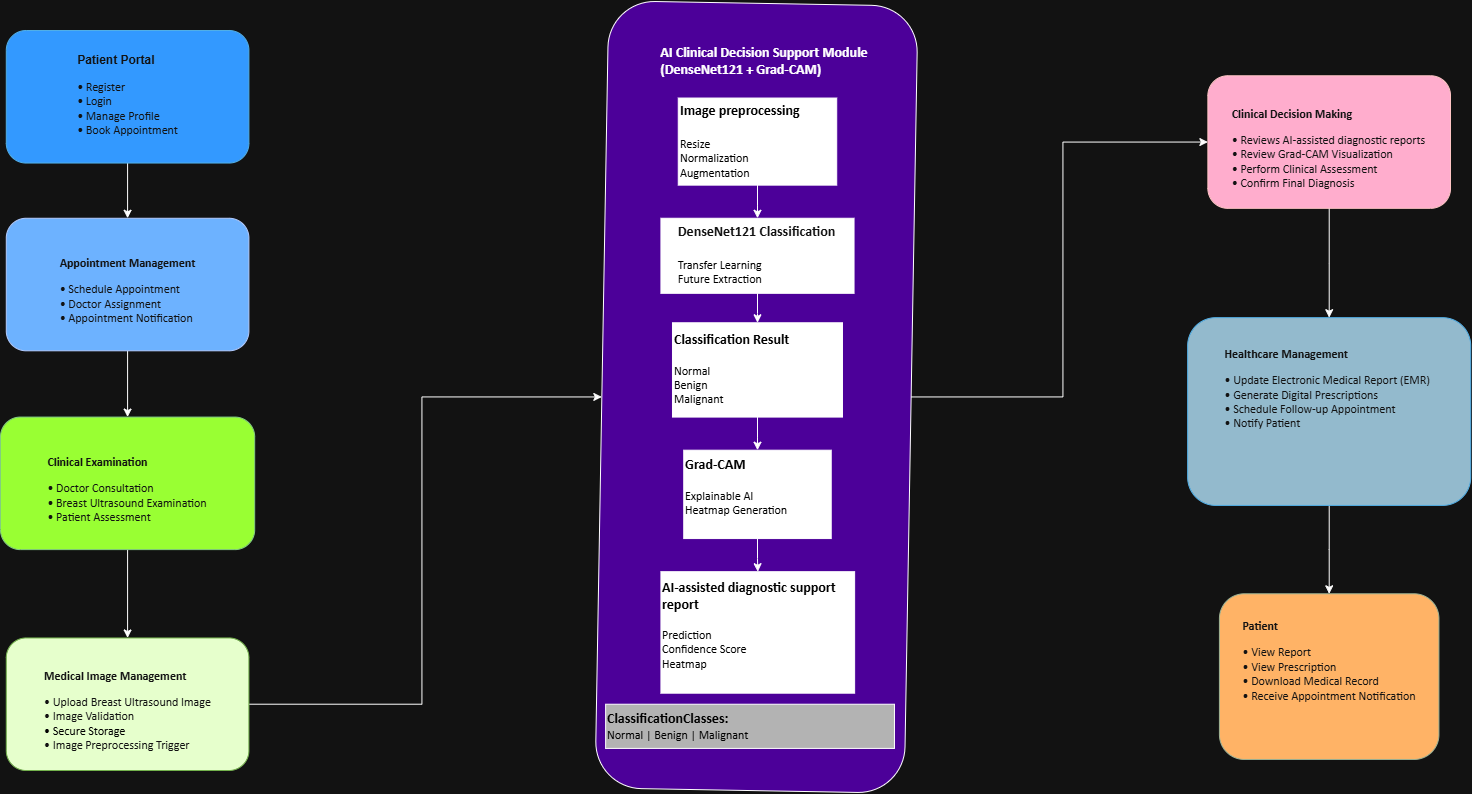
\includegraphics[width=\textwidth]{Workflow.png}
    \caption{System Workflow: Patient Journey and AI-Assisted Diagnostic Pipeline}
\end{figure}

\section{Software Architecture Overview}

 \textbf{RESTful APIs}.The diagram below illustrates the end-to-end workflow of the system, from patient interaction through AI-assisted diagnosis to final clinical and administrative follow-up.

\begin{figure}[H]
    \centering
    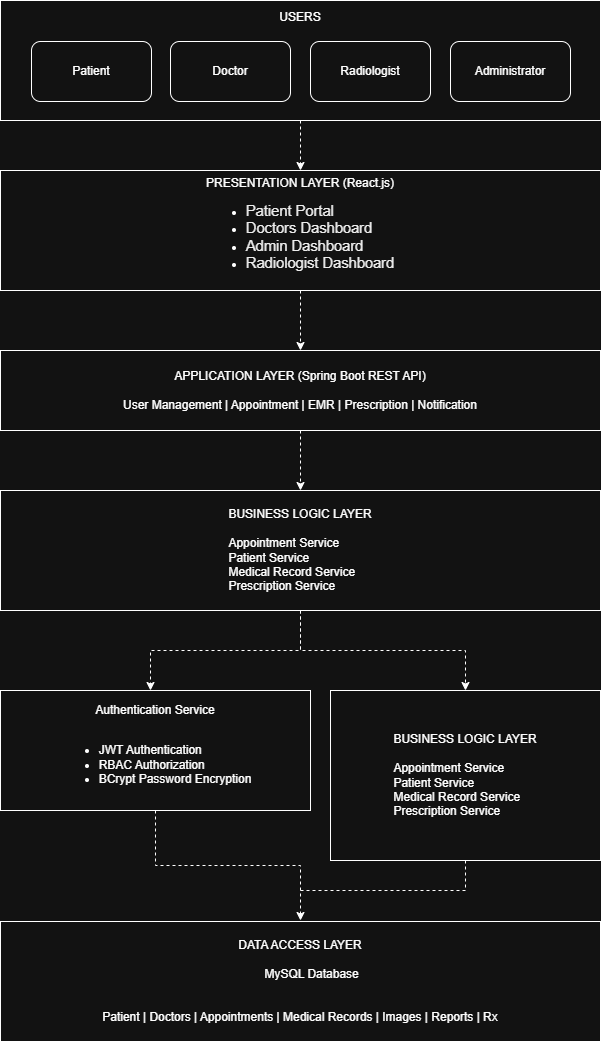
\includegraphics[width=0.65\textwidth]{Systematic achitecture.drawio.png}
    \caption{System Architecture Diagram}
\end{figure}

\section{Technologies Used}

\begin{itemize}[noitemsep]
    \item \textbf{React.js} -- Develop the responsive web-based user interface.
    \item \textbf{Spring Boot} -- Develop backend services and RESTful APIs.
    \item \textbf{MySQL} -- Store patient records, appointments, and healthcare data.
    \item \textbf{TensorFlow/Keras} -- Implement and train the deep learning model.
    \item \textbf{DenseNet121} -- Perform transfer learning for breast ultrasound image classification.
    \item \textbf{Grad-CAM} -- Provide Explainable AI (XAI) visualization for AI predictions.
    \item \textbf{JWT} -- Secure user authentication.
    \item \textbf{RBAC} -- Control system access based on user roles.
    \item \textbf{RESTful API} -- Enable communication between frontend, backend, and AI services.
    \item \textbf{Docker} -- Support application deployment and portability.
    \item \textbf{Google Colab} -- Train and evaluate the AI model using free GPU resources.
\end{itemize}
\section{Dataset Description}

The AI-assisted clinical decision support module will be developed using the \textbf{Breast Cancer Ultrasound Images (BUSI) Dataset}, obtained from the Hugging Face repository. The dataset contains labeled breast ultrasound images categorized into three classes: \textbf{Normal}, \textbf{Benign}, and \textbf{Malignant}, making it suitable for supervised deep learning-based image classification. The dataset will be used to train and evaluate a transfer learning model based on DenseNet121. Explainability will be achieved by applying Grad-CAM to visualize the image regions that contribute most to the model's predictions, thereby supporting clinicians in interpreting AI-generated results.

\section{Expected Benefits}

\subsection*{Benefits for Patients}

\begin{itemize}[noitemsep]
    \item Convenient online appointment scheduling.
    \item Secure access to electronic medical records.
    \item Digital prescriptions and healthcare reports.
    \item Faster access to AI-assisted clinical decision support.
\end{itemize}

\subsection*{Benefits for Healthcare Professionals}
\begin{itemize}[noitemsep]
    \item Centralized patient information.
    \item AI-assisted support for breast ultrasound interpretation.
    \item Explainable AI predictions using Grad-CAM.
    \item Improved clinical workflow and decision-making.
\end{itemize}

\subsection*{Benefits for Healthcare Organizations}
\begin{itemize}[noitemsep]
    \item Reduced paperwork and administrative workload.
    \item Improved operational efficiency.
    \item Secure management of healthcare data.
    \item Scalable and maintainable software architecture.
    \item Enhanced quality of healthcare services through integrated patient management and AI-assisted clinical decision support.
\end{itemize}


The use case diagram below illustrates the interactions between the four system actors, Patient, Doctor, Radiologist, and Administrator, and the core system functions, including appointment booking, medical record access, AI-assisted breast ultrasound classification, and administrative management.

\begin{figure}[h]
    \centering
    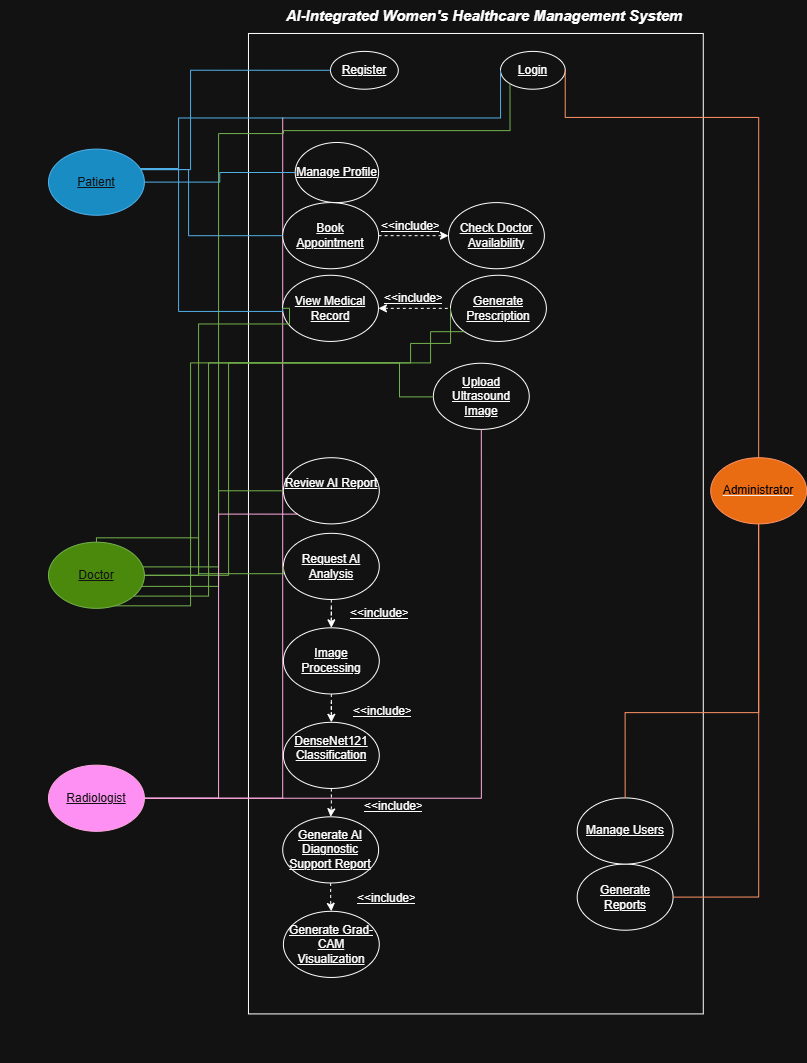
\includegraphics[width=\textwidth]{Case diagram.drawio (4).png}
    \caption{Use Case Diagram}
\end{figure}

% ============================================================
\chapter{Development Methodology}

\section{Selected Software Development Methodology}

The planned AI-Integrated Women's Healthcare Management System with Breast Cancer Diagnostic Support will develop by using the Agile Scrum methodology because it supports iterative and incremental development and allow the system to evolve through short development cycles called sprints. Scrum is well fit for this project because it allows continuous stakeholder feedback, regular testing and flexible adaptation to changing requirements. The system integrates Deep Learning for breast cancer diagnosis and Grad-CAM for explainable AI, both of which require continuous review and adjustment so by developing and testing modules incrementally, Scrum improves software quality, reduces development risks and ensures the final system meets both healthcare and technical requirements.
\begin{figure}[H]
    \centering
    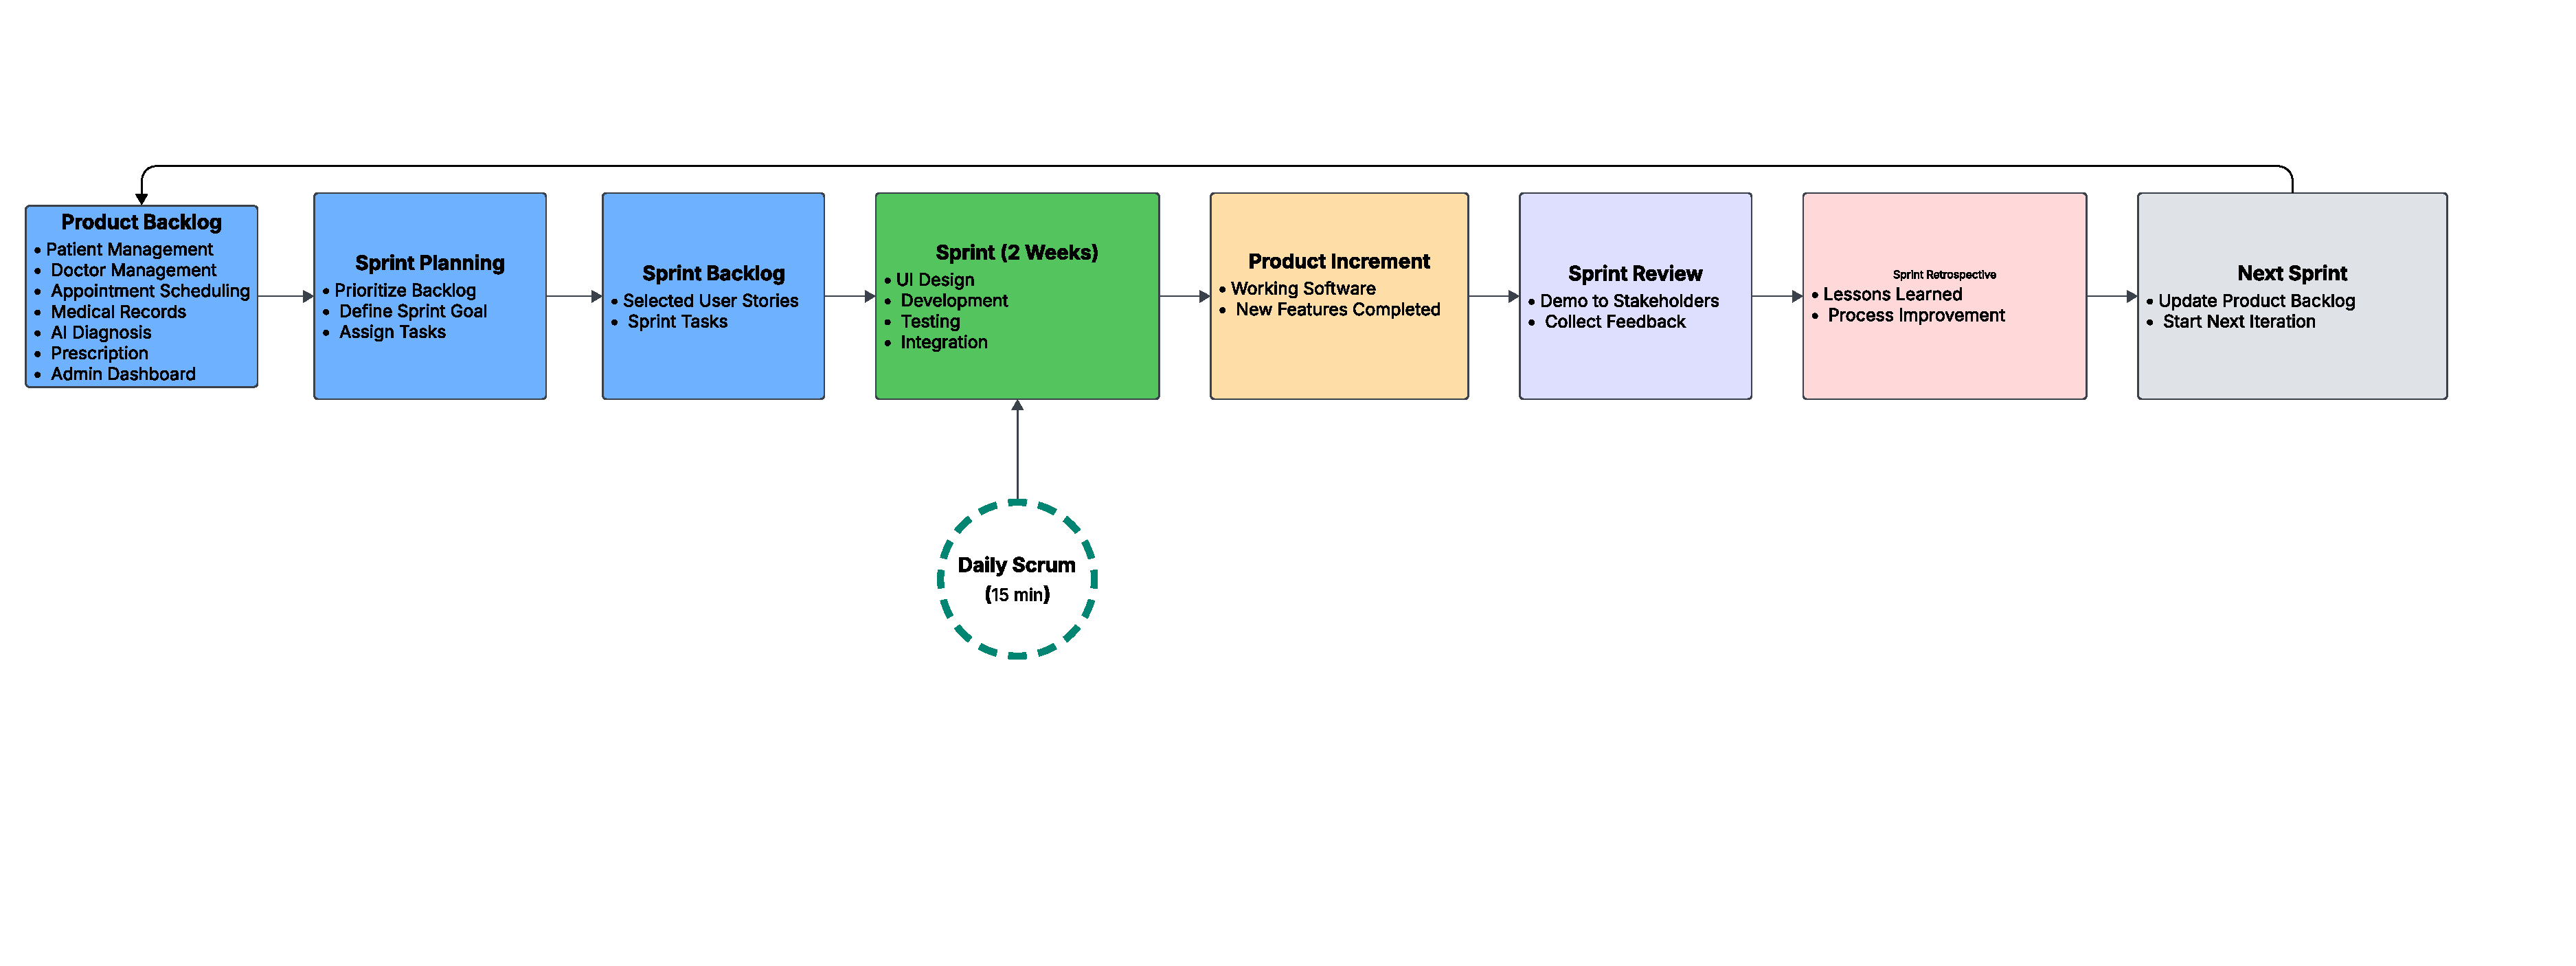
\includegraphics[width=0.9\textwidth]{agile.pdf}
    \caption{Agile Scrum Workflow for the AI-Integrated Women's Healthcare Management System with Breast Cancer Diagnostic Support}
    \label{fig:agile_scrum_workflow}
\end{figure}
This figure illustrates the Agile Scrum workflow adopted for this system and the development process begins with the Product Backlog that followed by Sprint Planning, Development, Testing, Sprint Review, and Sprint Retrospective in an iterative cycle. This workflow supports continuous improvement, stakeholder feedback and incremental delivery of the AI-Integrated Women's Healthcare Management System with Breast Cancer Diagnostic Support.
\subsection{Justification for Selecting Agile Scrum}

The Agile Scrum framework is selected for the following reasons:

\begin{enumerate}
\item \textbf{Continuous Improvement of the AI Model}

This system uses DenseNet121 for breast cancer classification and Grad-CAM for explainable AI and the Scrum supports iterative development, allowing the AI model to be continuously trained, tested and improved after each sprint.

\item \textbf{Continuous Stakeholder Feedback}

The system involves patients, doctors, radiologists and administrators that the Scrum will enable regular stakeholder feedback during sprint reviews, ensuring the system evolves according to user needs and clinical requirements.

\item \textbf{Modular and Incremental Development}

The system consists of independent modules such as authentication, patient management, appointments, medical records, AI diagnosis, prescriptions and administration, so scrum allows these modules to be developed, tested and integrated incrementally.

\item \textbf{Early Risk Identification and Mitigation}

Regular testing and sprint reviews help identify technical issues, security risks and AI performance limitations early, reducing development risks and minimizing costly changes.

\item \textbf{Higher Software Quality through Continuous Testing}

Each sprint includes testing and evaluation to verify system functionality, integration, usability and AI performance that the Continuous testing improves software reliability and ensures the system performs effectively before deployment.
\end{enumerate}
\begin{figure}[H]
    \centering
    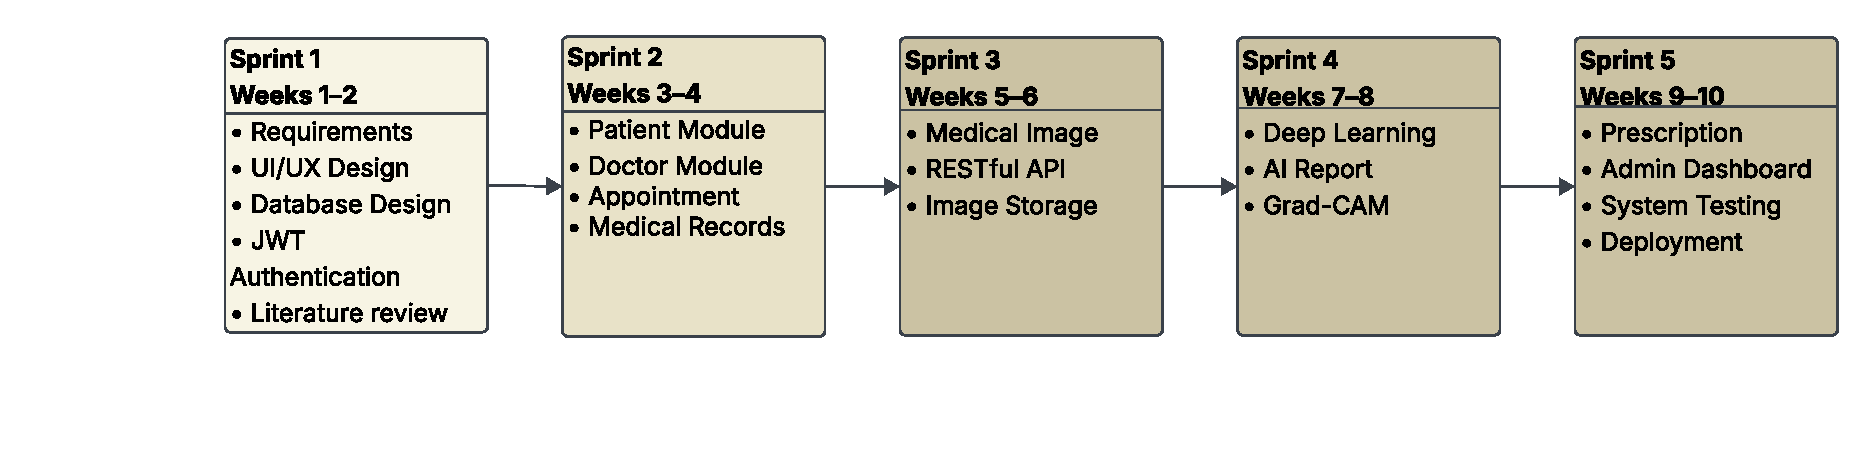
\includegraphics[width=0.9\textwidth]{sprint.pdf}
    \caption{Sprint Timeline for the AI-Integrated Women's Healthcare Management System with Breast Cancer Diagnostic Support}
    \label{fig:agile_scrum_workflow}
\end{figure}
Figure 1.2 presents the planned sprint timeline for developing the AI-Integrated Women's Healthcare Management System that each sprint focuses on implementing and testing specific modules including patient management, medical image processing, AI-assisted diagnosis and system deployment. This iterative schedule enables continuous integration, testing and refinement throughout the development process.


% ============================================================
\chapter{Requirement Elicitation}

\section{Requirement Gathering Approach}

The selected topic AI-Integrated Women's Healthcare Management System with Breast Cancer Diagnostic Support implements a multi-technique requirement elicitation approach to ensure comprehensive and precise requirement collection and the system involves multiple stakeholders, including patients, doctors, radiologists, and administrators, requirements that will be gathered through interviews, questionnaires, direct observation and Joint Application Development (JAD) sessions, so these techniques gives detailed clinical insights, user expectations, collaborative decision-making and a better understanding of existing healthcare workflows. The collected requirements will then be analyzed, validated, prioritized, and documented in the Software Requirements Specification (SRS) to support the iterative development process using the Agile Scrum methodology.
\begin{figure}[H]
    \centering
    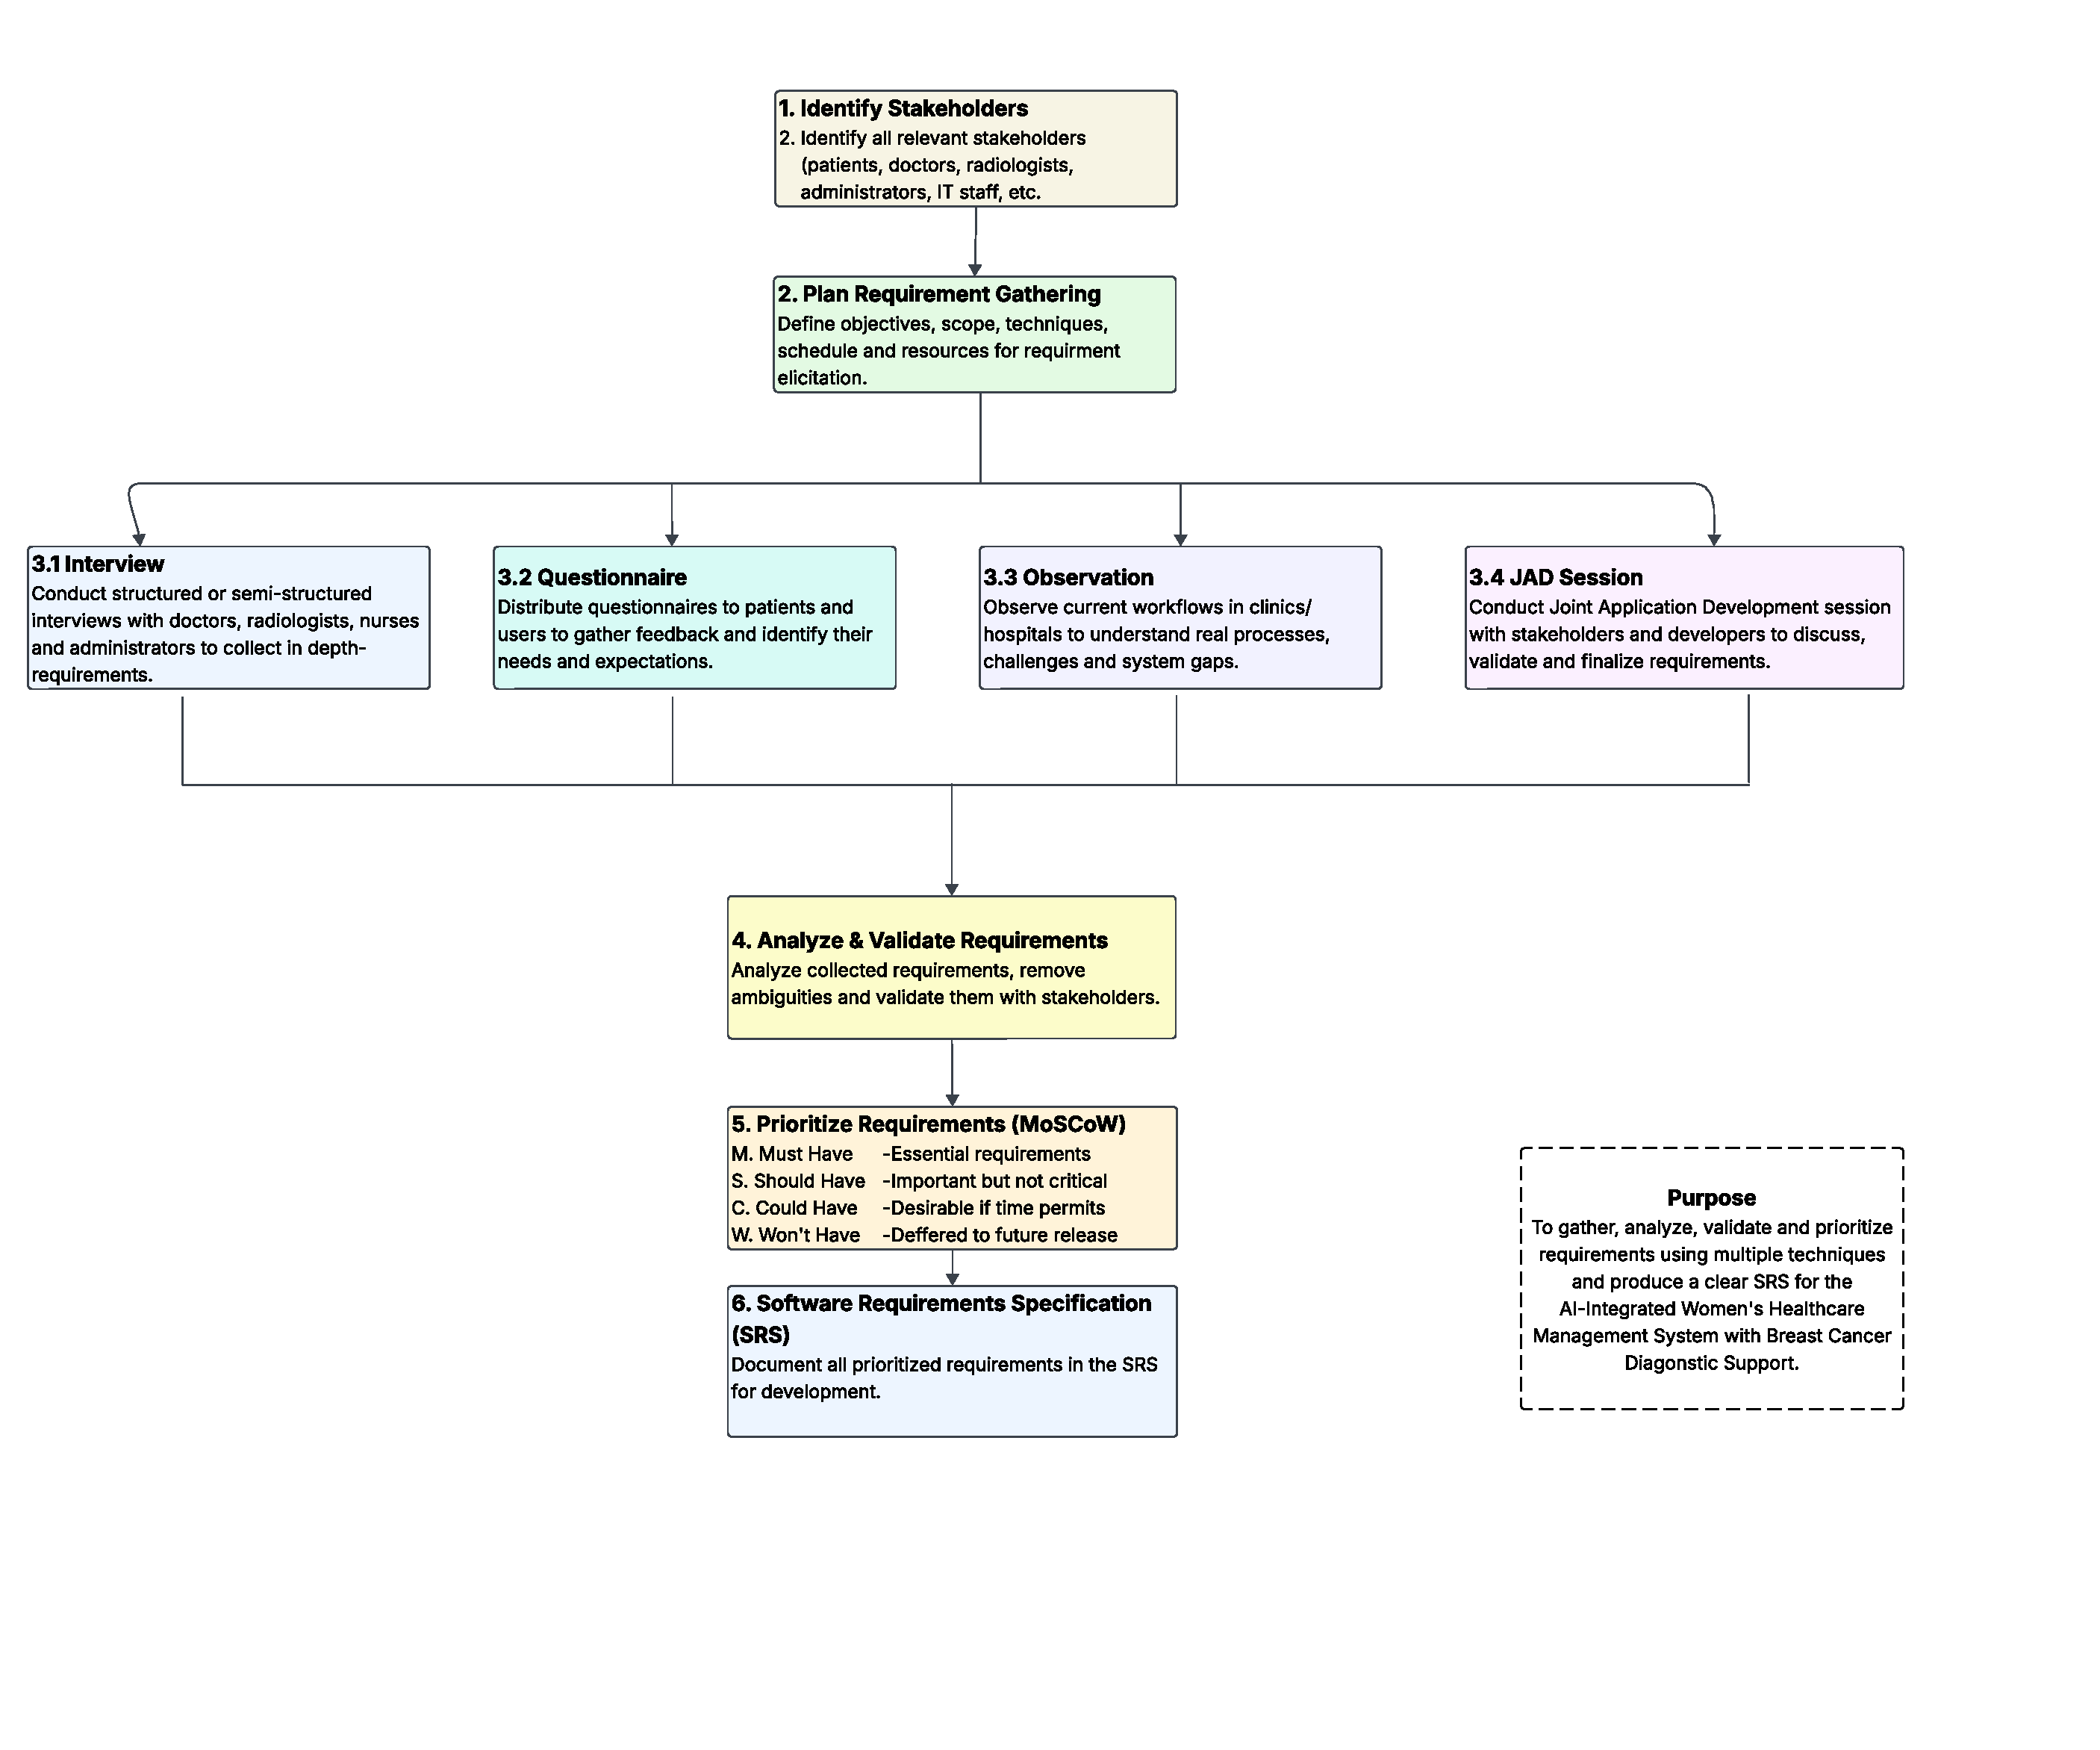
\includegraphics[width=0.9\textwidth]{elicitation.pdf}
    \caption{Requirement Elicitation Workflow for the AI-Integrated Women's Healthcare Management System with Breast Cancer Diagnostic Support}
    \label{fig:agile_scrum_workflow}
\end{figure}
Figure 1.3 shows the requirement elicitation workflow selected for the system and the requirements are gathered through interviews, questionnaires, observation, and JAD sessions so then analyzed and documented in the Software Requirements Specification (SRS). This structured process ensures that stakeholder needs are accurately captured before system development begins.

\subsection{Requirement Elicitation Plan}

\begin{table}[H]
\centering





\caption{Requirement Elicitation Plan}
\begin{tabular}{|p{3cm}|p{3.5cm}|p{3.5cm}|p{4cm}|}
\hline
\textbf{Activity} & \textbf{Stakeholders} & \textbf{Purpose} & \textbf{Expected Outcome} \\
\hline
Interview & Doctors, Radiologists & Gather clinical requirements & Functional requirements \\
\hline
Questionnaire & Patients & Collect user expectations & User requirements \\
\hline
Observation & Hospital Staff & Understand workflow & Workflow requirements \\
\hline
JAD Session & Doctors, Admin, Developers & Validate requirements & Final agreed requirements \\
\hline
\end{tabular}
\end{table}

\subsection{Interviews}

Semi-structured interviews will be conducted with doctors and radiologists because they support the domain knowledge necessary to define the clinical workflow and system requirements. The interviews will focus on understanding current practices in breast cancer diagnosis, patient record management, appointment scheduling, identifying limitations of existing healthcare systems, and determining how AI-assisted decision support can enhance clinical efficiency. This interviews are selected because they allow predefined questions while providing the flexibility to explore additional issues raised by participants.

\begin{table}[H]
\centering
\caption{Interview Questions}
\begin{tabular}{|c|p{12cm}|}
\hline
\textbf{No.} & \textbf{Interview Question} \\
\hline
1 & What challenges do you currently face when diagnosing breast cancer using ultrasound images? \\
\hline
2 & How are patient medical records currently managed? \\
\hline
3 & What information should an AI-assisted diagnostic report contain? \\
\hline
4 & How should ultrasound images be uploaded and stored? \\
\hline
5 & Would Grad-CAM visualizations improve your confidence in AI predictions? Why? \\
\hline
6 & What prescription information should the system generate automatically? \\
\hline
7 & What security and privacy measures should the system implement? \\
\hline
8 & What features are essential for appointment scheduling? \\
\hline
9 & What administrative reports would be useful? \\
\hline
10 & What additional features would improve your daily clinical workflow? \\
\hline
\end{tabular}
\end{table}



\subsection{Questionnaire}

A structured questionnaire will be given to patients to know better of their expectations regarding digital healthcare services and it focuses on usability, accessibility, appointment scheduling, electronic medical records, AI-assisted diagnosis and data privacy that the responses will be collected using a five-point Likert scale ranging from Strongly Disagree (1) to Strongly Agree (5).

\begin{table}[H]
\centering
\caption{Patient Questionnaire}
\begin{tabular}{|c|p{10cm}|c|}
\hline
\textbf{No.} & \textbf{Questionnaire Statement} & \textbf{Scale} \\
\hline
1 & The system should be easy to use. & 1--5 \\
\hline
2 & Online appointment scheduling would improve healthcare services. & 1--5 \\
\hline
3 & I would like secure online access to my medical records. & 1--5 \\
\hline
4 & AI-assisted diagnosis would increase healthcare efficiency. & 1--5 \\
\hline
5 & AI-generated diagnostic reports should be reviewed by doctors before use. & 1--5 \\
\hline
6 & Protecting my medical data and privacy is important. & 1--5 \\
\hline
7 & Receiving digital prescriptions would be convenient. & 1--5 \\
\hline
8 & Overall, I would be willing to use this healthcare system. & 1--5 \\
\hline
\end{tabular}
\end{table}

\subsection{JAD Session}

Joint Application Development (JAD) sessions will be taken to show the validate of the collected requirements and determine any overlapping stakeholder expectations and it encourages collaboration among doctors, radiologists, hospital administrators and the development team will ensure that the proposed system satisfies clinical needs, technical feasibility, and user expectations.

\begin{table}[H]
\centering
\caption{JAD Session Plan}
\begin{tabular}{|p{3.5cm}|p{4cm}|p{3cm}|p{4cm}|}
\hline
\textbf{Activity} & \textbf{Participants} & \textbf{Purpose} & \textbf{Expected Outcome} \\
\hline
Review project objectives & All participants & Introduce the project scope & Shared understanding \\
\hline
Discuss functional requirements & Doctors, Radiologists, Developers & Validate system features & Agreed functional requirements \\
\hline
Discuss non-functional requirements & Administrators, Developers & Identify security, privacy, and performance needs & Validated non-functional requirements \\
\hline
Resolve requirements conflicts & All participants & Reach consensus & Finalized requirements \\
\hline
Prioritize requirements & All participants & Identify implementation priorites & Prioritized requirement list \\
\hline
\end{tabular}
\end{table}

\subsection{Observation}

Direct observation will be conducted within healthcare facilities to know the existing clinical workflow and the development team will observe patient registration, appointment scheduling, doctor consultations, ultrasound image handling and prescription generation, the observation will help to identify workflow inefficiencies and practical requirements that may not be fully captured through interviews or questionnaires.

\begin{table}[H]
\centering
\caption{Observation Plan}
\begin{tabular}{|p{4cm}|p{3.5cm}|p{3cm}|p{4cm}|}
\hline
\textbf{Activity Observed} & \textbf{Stakeholders} & \textbf{Purpose} & \textbf{Expected Outcome} \\
\hline
Patient registration & Reception staff, Patients & Understand registration workflow & Registration requirements \\
\hline
Appointment scheduling & Reception staff, Patients & Analyze scheduling process & Appointment management requirements \\
\hline
Doctor consultation & Doctors, Patients & Observe diagnosis workflow & Clinical workflow requirements \\
\hline
Ultrasound image handling & Radiologists & Study image upload workflow & Prescription management requirements \\
\hline
Prescription process & Doctors, Pharmacists & Understand prescription workflow & Prescription management requirements \\
\hline
\end{tabular}
\end{table}

% ============================================================
\chapter{Project Planning}

\section{Work Breakdown Structure and Activity List}

TSo, the project plan for the AI-Integrated Women’s Healthcare Management System, with Explainable Breast Cancer Clinical Decision Support, kind of starts by getting a Work Breakdown Structure, (WBS) together and also building an activity list. The WBS sorts the whole effort into five big phases Project Planning, Design and Development, Testing and Quality Assurance, Implementation and Deployment, and finally Project Closure. After that each phase gets broken into more specific tasks and activities, so it’s easier for everyone to handle planning, scheduling, keeping an eye on progress, and general project control. The activity list then pulls everything into one sequence, with expected time frames, their dependencies, and how each step links to the next, which gives a pretty solid map for finishing the project properly, not just… kind of thinking about it.


\begin{figure}[H]
\centering
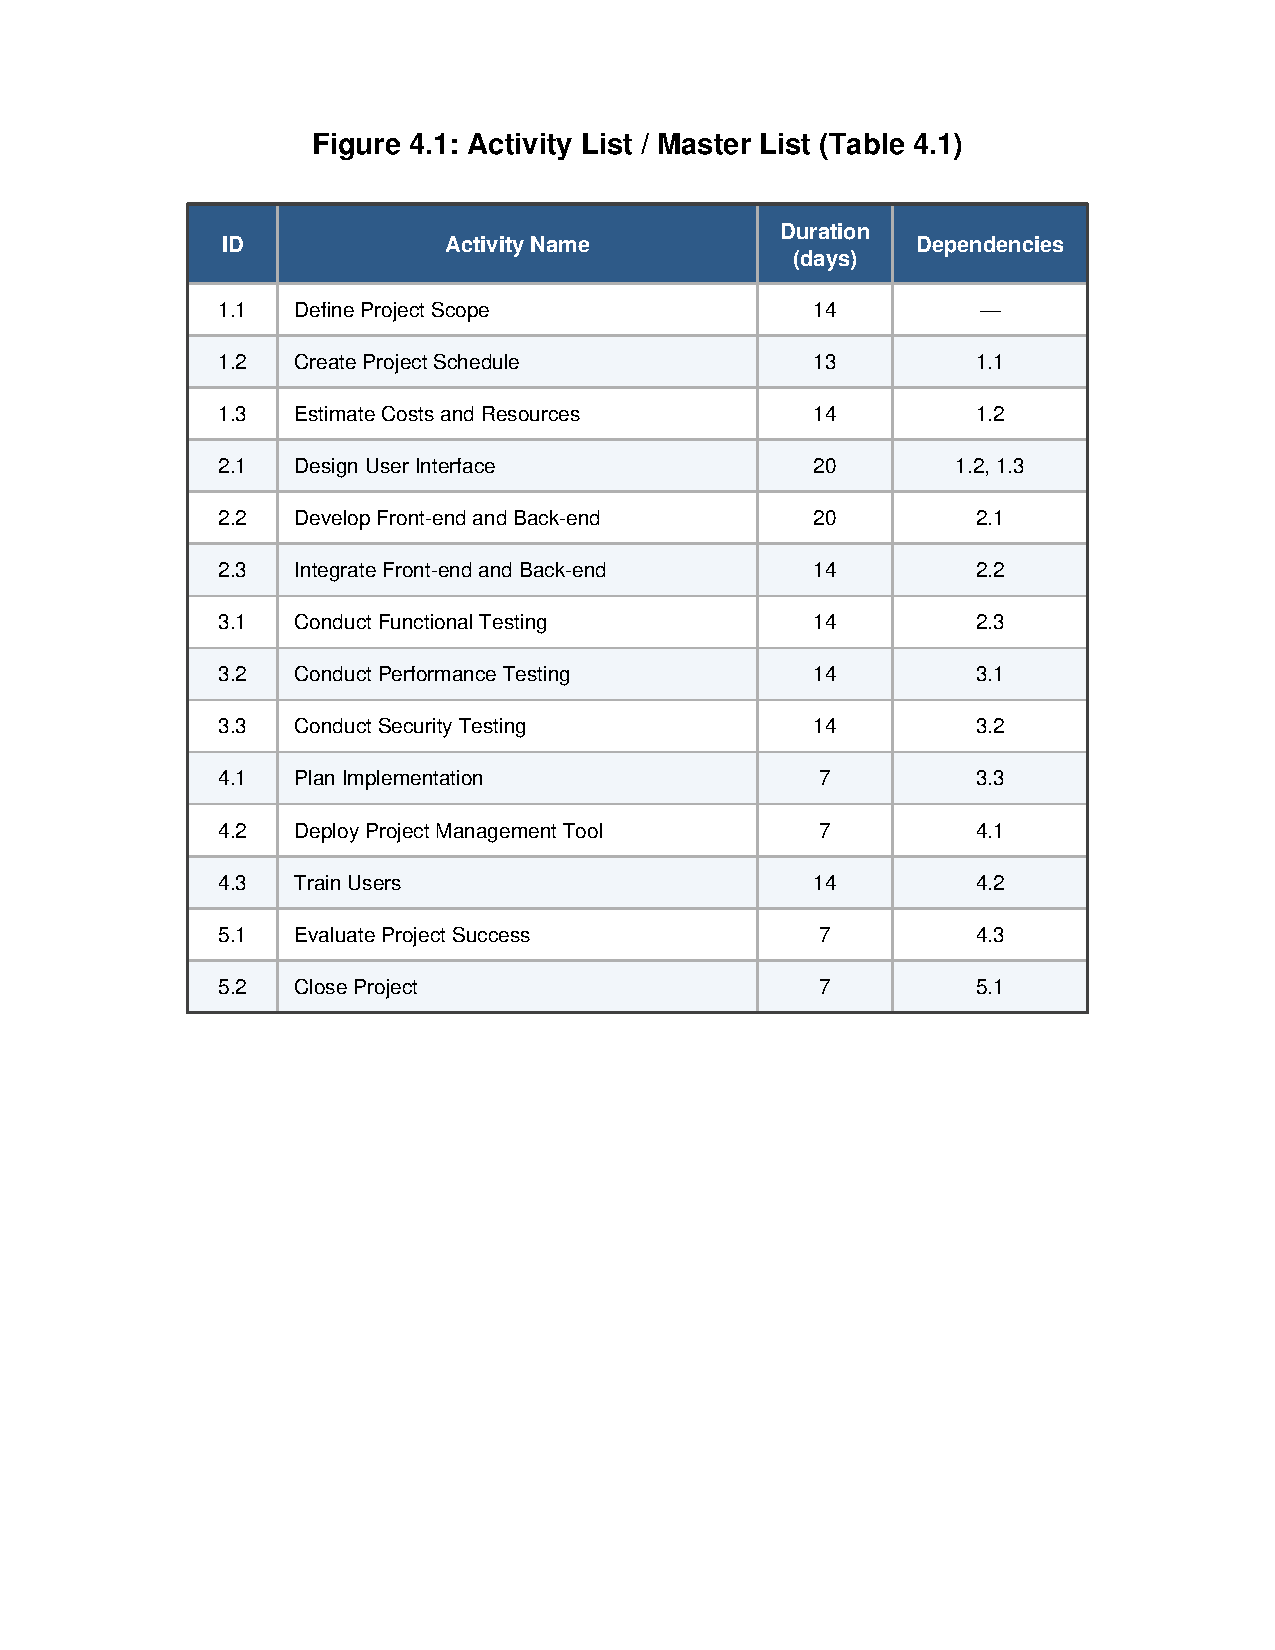
\includegraphics[width=\textwidth]{Figure_4.1_Activity_List (1).pdf}

\caption{Activity List / Master List (Table 4.1)}
\end{figure}

\begin{figure}[H]
\centering
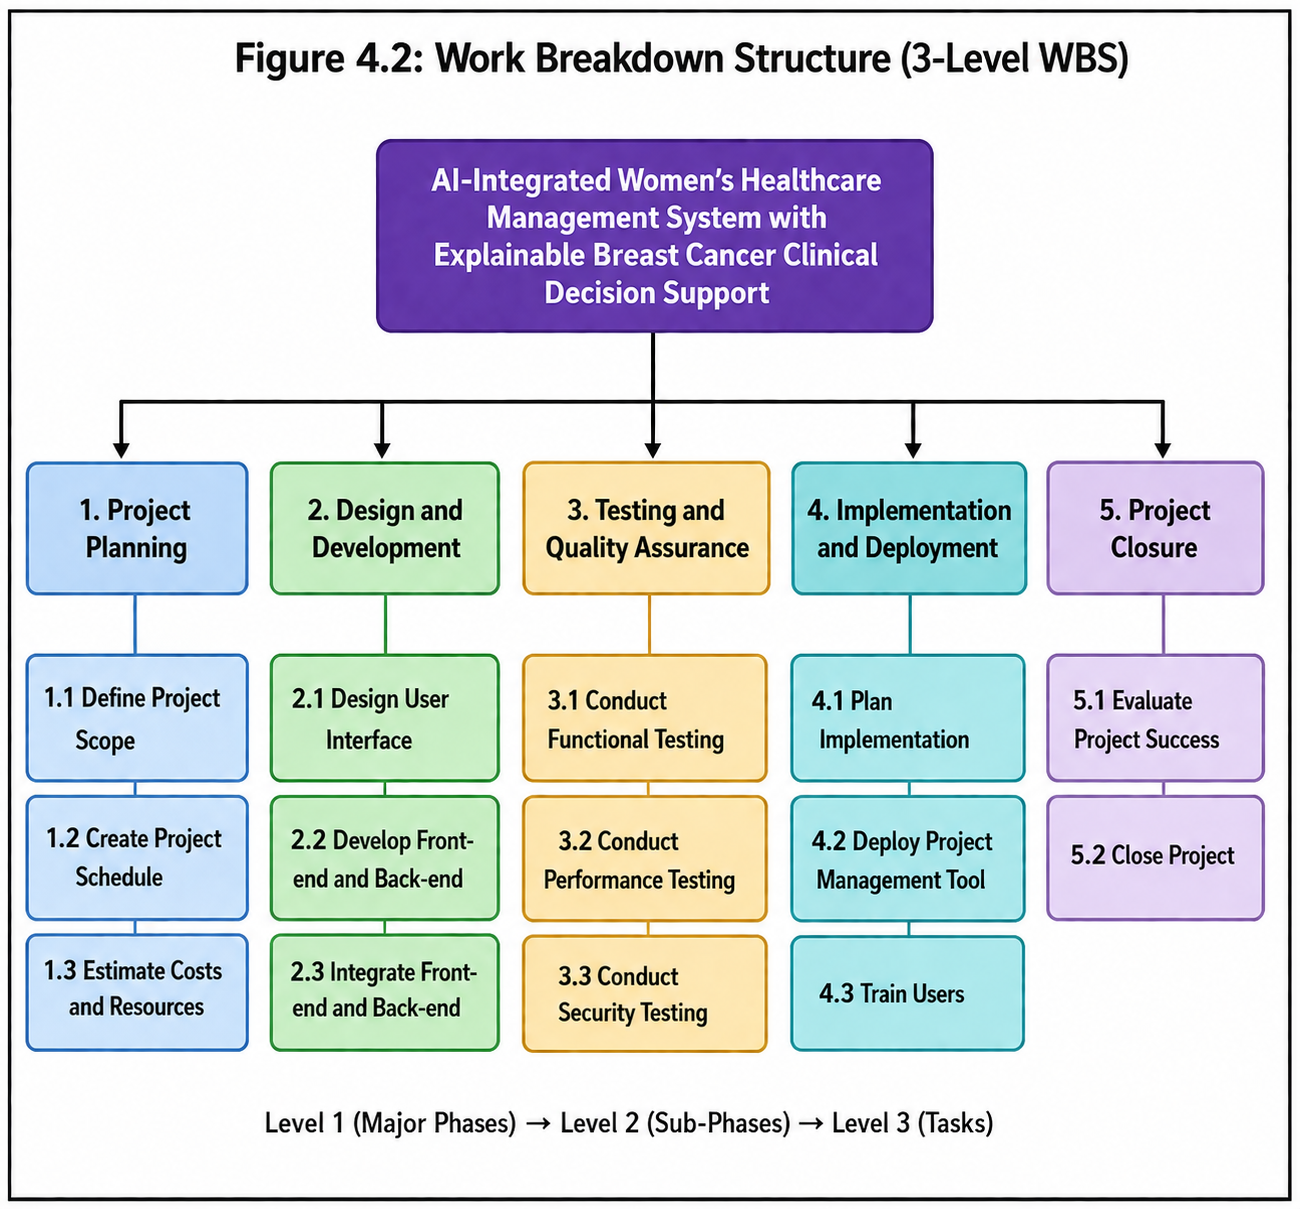
\includegraphics[width=\textwidth]{4.2..png}
\caption{Work Breakdown Structure (3-Level WBS)}
\end{figure} 



\section{Gantt Chart}

The Gantt chart shows the general timing for the AI-Integrated Women’s Healthcare Management System project, you can kind of see the big picture from it. It displays the start date, end date, duration, and also the order, of each project activity. The schedule kicks off with project planning, then goes into system design, after that development, integration, testing, implementation, later user training, evaluation, and finally project closure. With this chart it becomes easier to watch how things are moving and to make sure the activities are actually wrapped up inside the planned timeline, more or less as expected.


\begin{figure}[H]
\centering
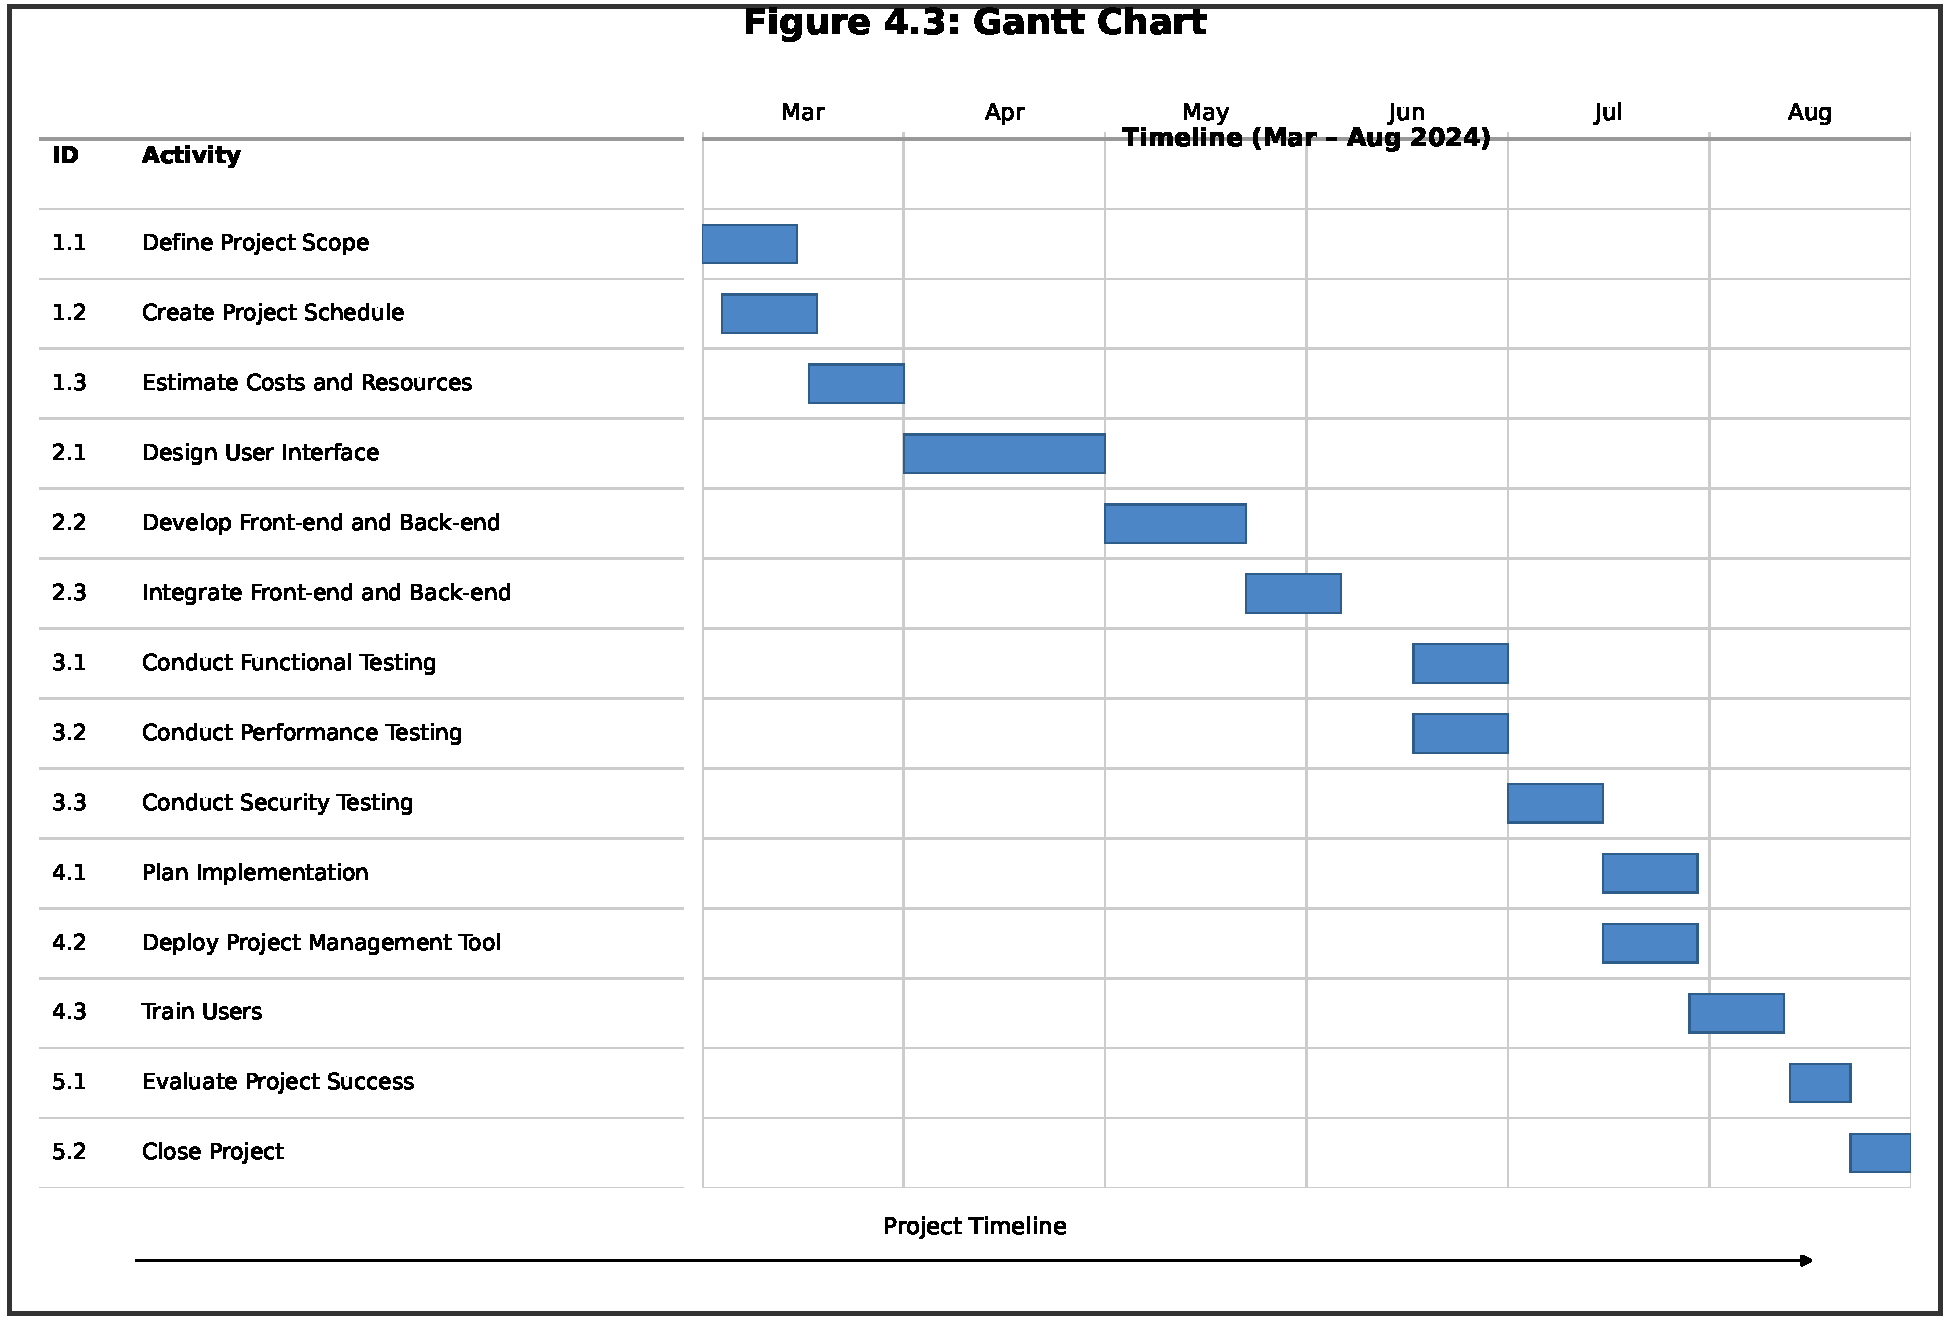
\includegraphics[width=\textwidth]{Figure_4.3_Gantt (1).pdf}
\caption{Gantt Chart}
\end{figure}


\section{Network Diagram, Critical Path, and Slack Time Analysis}

The diagram of the network, critical path review, and the slack time check were put together to judge the project schedule for the AI-Integrated Women’s Healthcare Management System with Explainable Breast Cancer Clinical Decision Support. In general these kinds of planning approaches show the order of project tasks, point out which tasks directly touch the end date, and also clarify if any activities could be postponed, without messing up the whole schedule.

\section{Network diagram} 

Figure 4.4 shows the network diagram for the project. It sort of illustrates the logical tie between all the project activities, starting at defining the project scope and finishing at project closure. In other words, you can see how each activity depends on whether the previous activity is done, so it kind of gives a clear picture of the workflow and the execution order, for the whole project. 

\begin{figure}[H]
\centering
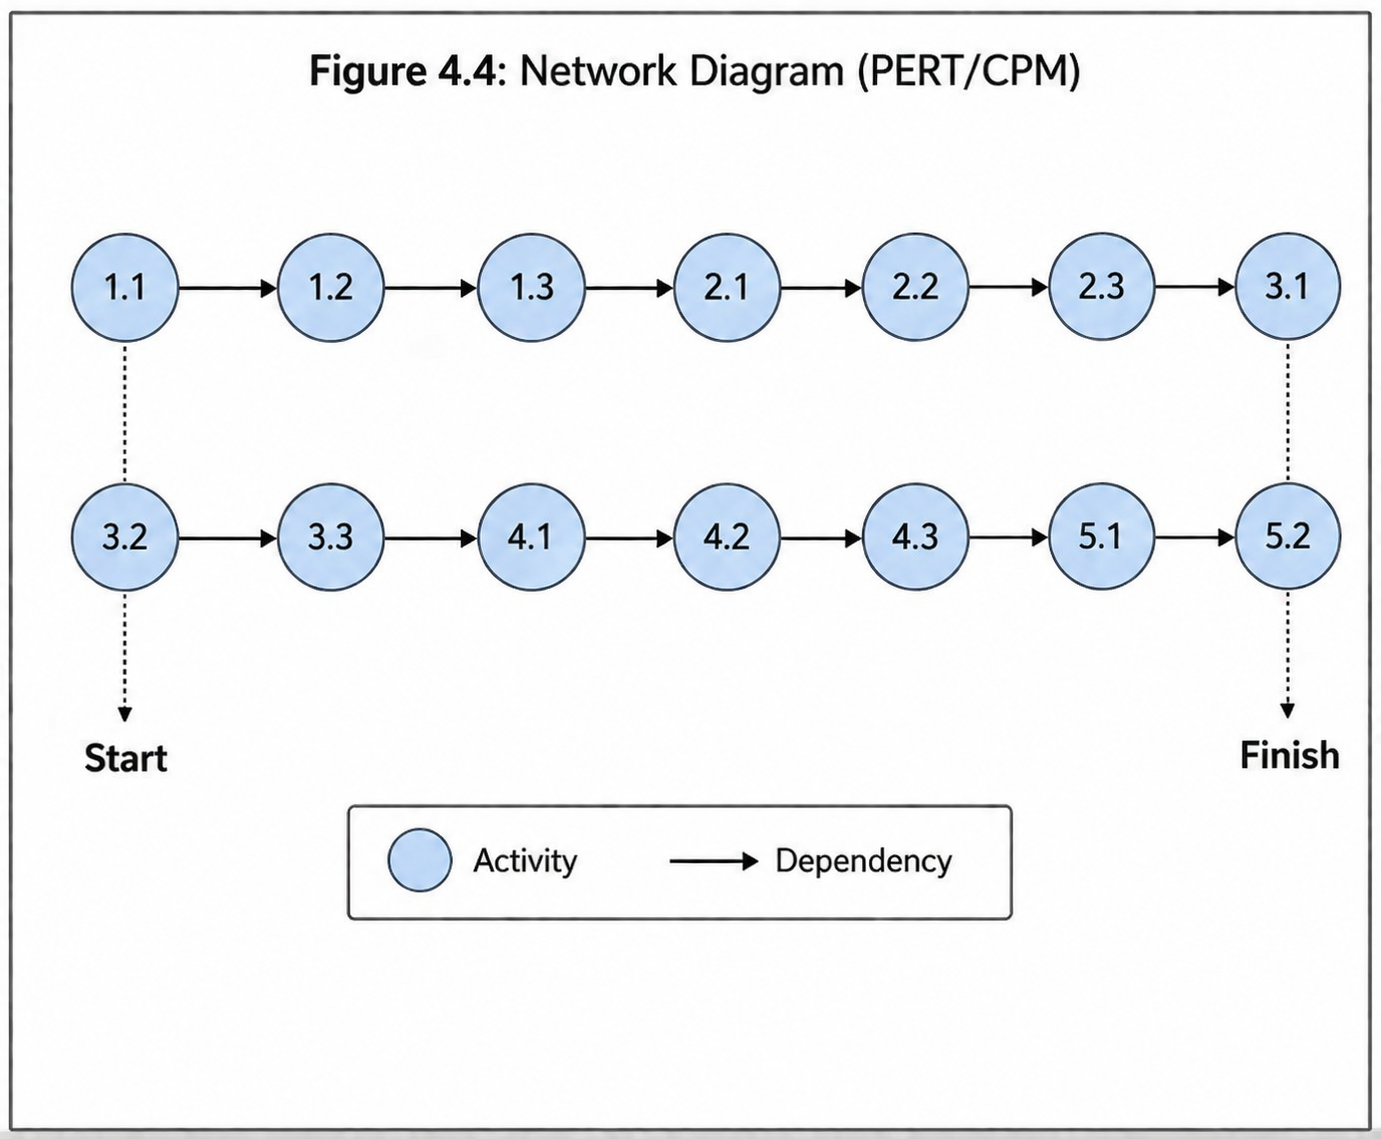
\includegraphics[width=\textwidth]{4.4..png}
\caption{Network Diagram (PERT/CPM)}
\end{figure}


\section{Critical Path Analysis} 

Figure 4.5 shows a kind of critical path analysis for the project, like where the whole timeline really hangs on. On that critical path there are activities such as Define Project Scope, Create Project Schedule, Estimate Costs and Resources, Design User Interface, Develop Front-end and Back-end, Integrate Front-end and Back-end, Conduct Functional Testing, Conduct Performance Testing, Conduct Security Testing, Plan Implementation, Deploy Project Management Tool, Train Users, Evaluate Project Success, and Close Project. All these items happen in sequence so they end up being the longest route across the project network, not just the “main” route. Because of that, if any one activity slips—even a bit—then the project completion date gets pushed back, kind of straight away.

\begin{figure}[H]
\centering
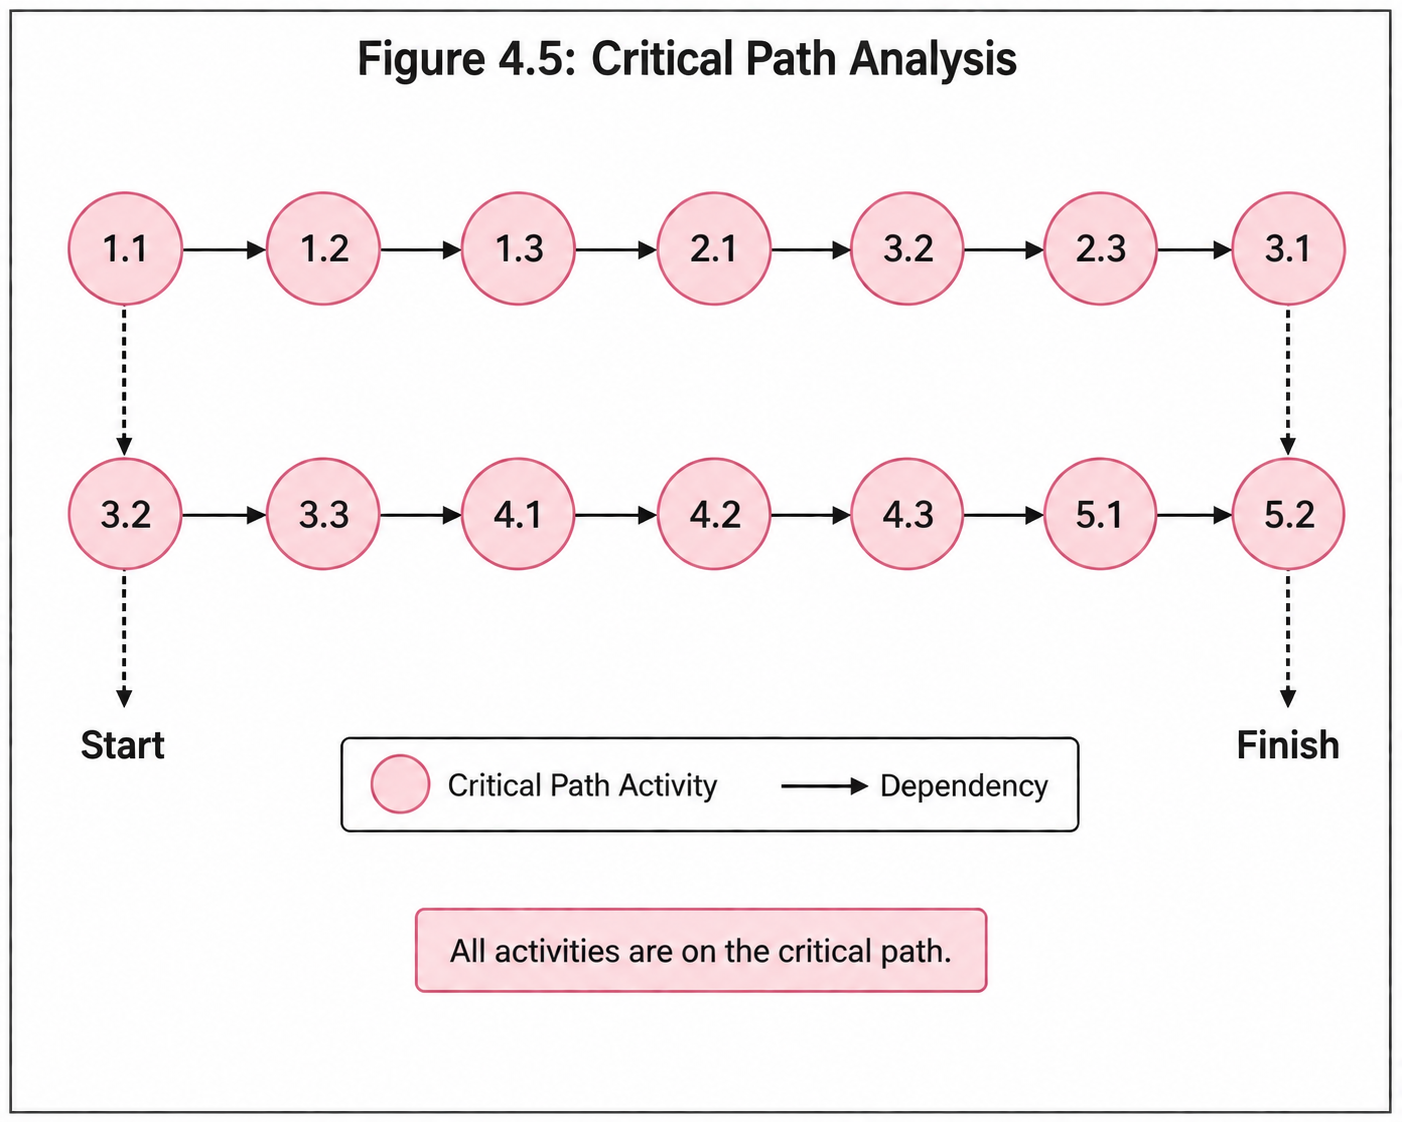
\includegraphics[width=\textwidth]{4.5..png}
\caption{Critical Path Analysis}
\end{figure}


\section{Slack time analysis} 

Figure 4.6 kinda shows the slack time analysis for the project activities, and if you look closely you’ll see it’s basically saying the same thing for each item. All of them end up with zero slack because every task is sitting directly on the critical path. They also seem to depend on the completion of the activity right before it, so nothing really gets a free buffer. Because of that, none of the activities can be pushed back, not really, without messing with the overall project completion date. So the main takeaway is that you really need to finish every project phase in line with the schedule that was planned, otherwise the whole timeline slips. 

\begin{figure}[H]
    \centering
    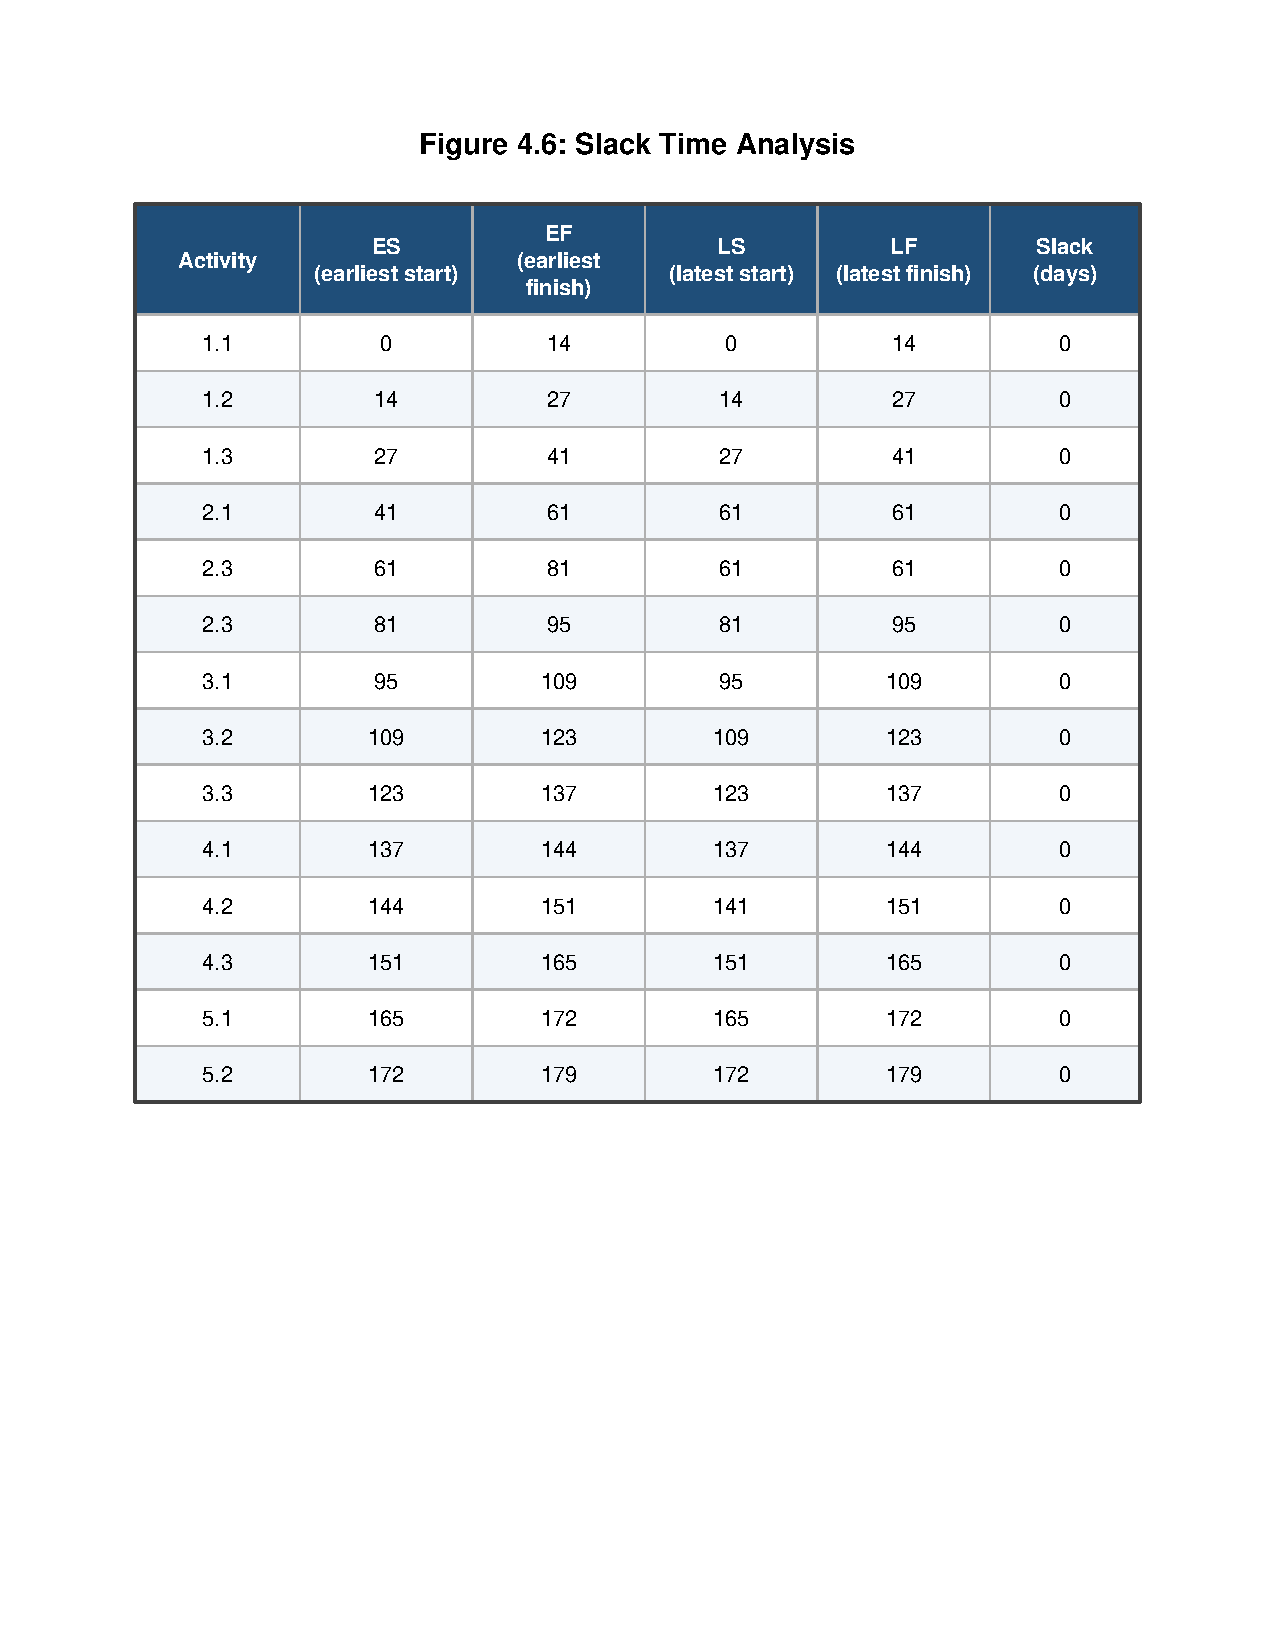
\includegraphics[width=\textwidth]{Figure_4.6_Slack_Time_Analysis.pdf}
    \caption{Slack Time Analysis}
\end{figure}

% ============================================================
\chapter{Cost and Benefit Analysis}

\section{Introduction}

Before starting any kind of software development, it’s essential to check whether the project is economically possible. Cost-Benefit Analysis (CBA) kind of answers the question of, if the expected benefits from the proposed system actually outweigh the investment needed for development and ongoing maintenance. And since the proposed \textbf{AI-Integrated Women's Healthcare Management System with Breast Cancer Diagnostic Support} blends healthcare management with Artificial Intelligence, the assessment also includes both tangible gains and intangible improvements.

The financial analysis usually covers the identification of project expenses, predicted benefits, Net Present Value (NPV), and Return on Investment (ROI). For academic use, fairly reasonable cost projections are taken, to show that the project feasibility holds up even in a more formal setting.

\section{Project Cost Components}

\begin{figure}[h]
    \centering
    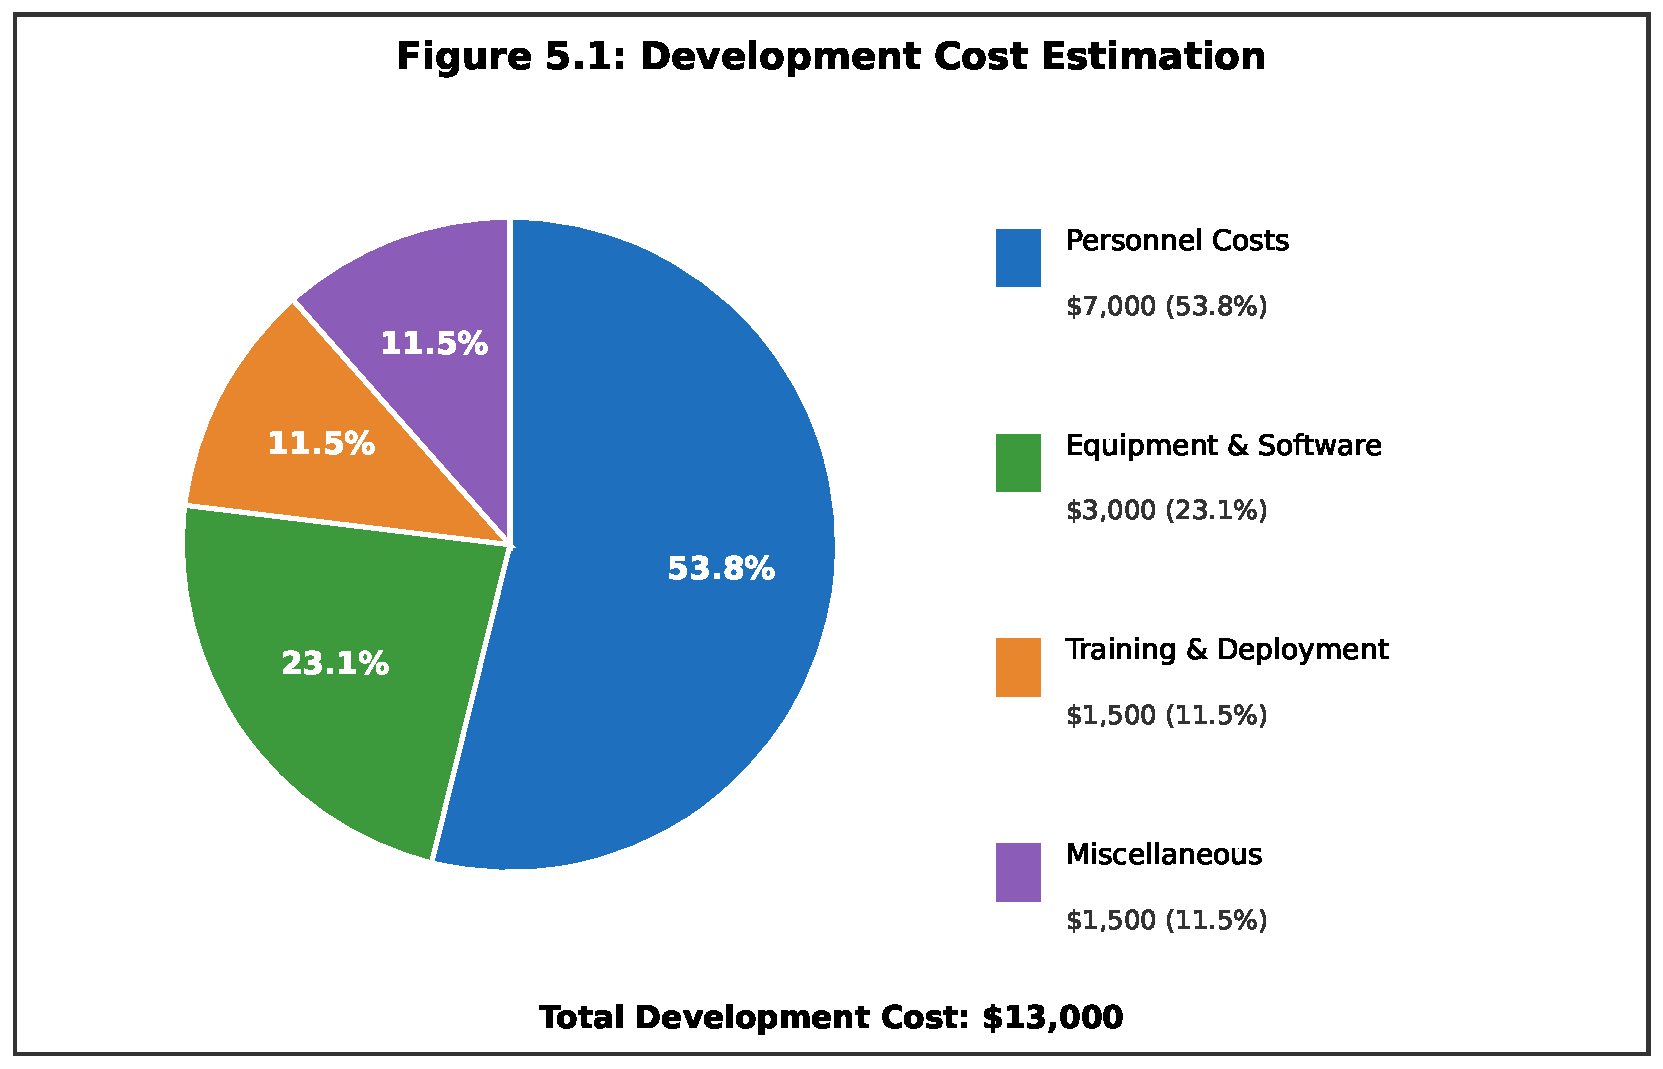
\includegraphics[width=0.8\textwidth]{Figure_5.1_Cost_Estimation.pdf}
    \caption{Development Cost Estimation (Table 5.1)}
\end{figure}

\section{Expected Benefits}

The proposed system provides both tangible and intangible benefits.

\subsection*{Tangible Benefits}
\begin{itemize}[noitemsep]
    \item Reduced administrative workload.
    \item Faster appointment scheduling.
    \item Reduced paper-based documentation.
    \item Improved operational efficiency.
    \item Reduced manual record management costs.
    \item Earlier diagnostic support that may improve workflow efficiency.
\end{itemize}

\subsection*{Intangible Benefits}
\begin{itemize}[noitemsep]
    \item Improved patient satisfaction.
    \item Enhanced clinical decision support.
    \item Better healthcare accessibility.
    \item Improved data security through JWT-based authentication and RBAC.
    \item Increased transparency using Grad-CAM explainability.
    \item Enhanced institutional reputation through AI-assisted healthcare services.
\end{itemize}

\section{Net Present Value (NPV) Analysis}

\subsection*{Assumptions}
\begin{itemize}[noitemsep]
    \item Initial Investment = \textbf{USD 13,000}
    \item Annual Benefit = \textbf{USD 8,000}
    \item Annual Operating Cost = \textbf{USD 3,000}
    \item Net Cash Flow = \textbf{USD 5,000/year}
    \item Discount Rate = \textbf{10\%}
    \item Project Duration = \textbf{5 Years}
\end{itemize}

\begin{figure}[!htbp]
    \centering
    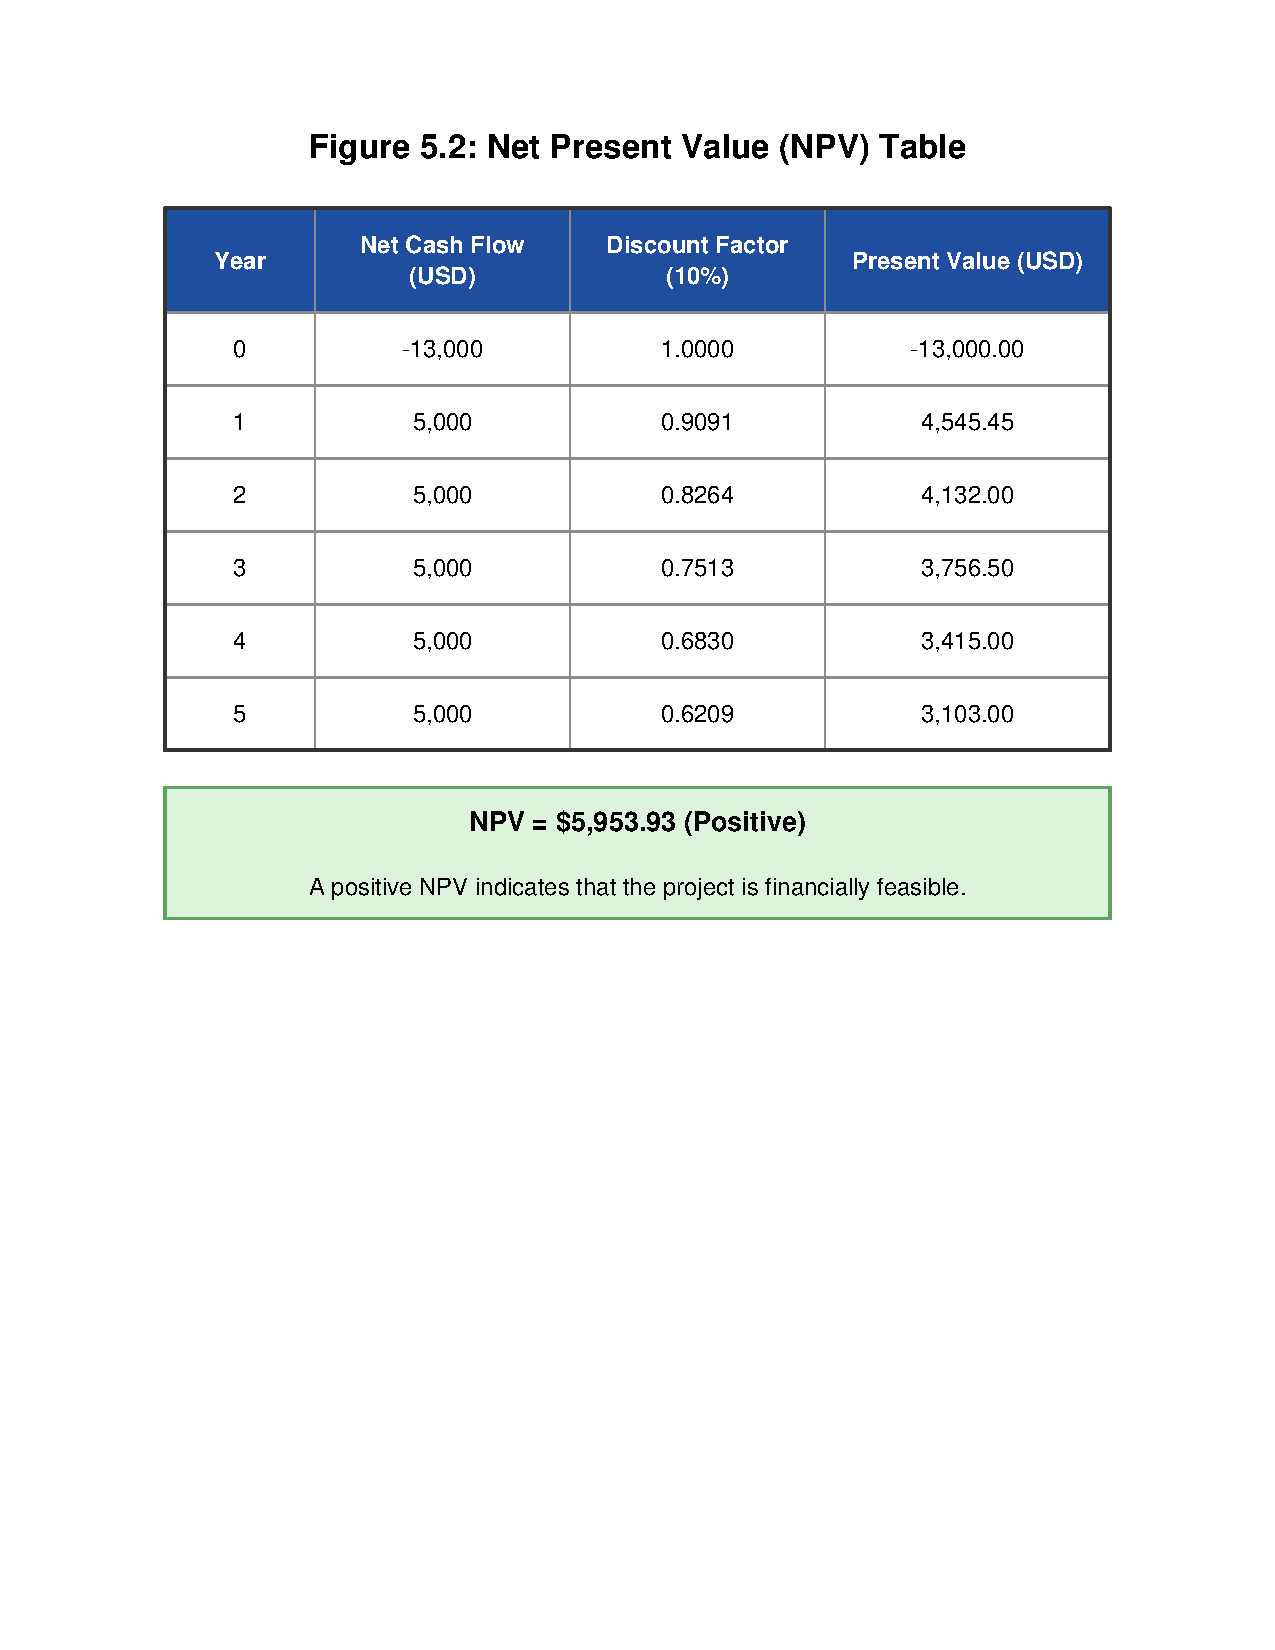
\includegraphics[
        width=0.65\textwidth,
        trim=1.5cm 1.5cm 1.5cm 1.5cm,
        clip
    ]{Figure_5.2_NPV_Table (2).pdf}
    \caption{Net Present Value (NPV) Table}
\end{figure}

\clearpage

\section{Return on Investment (ROI)}

\begin{figure}[!htbp]
    \centering
    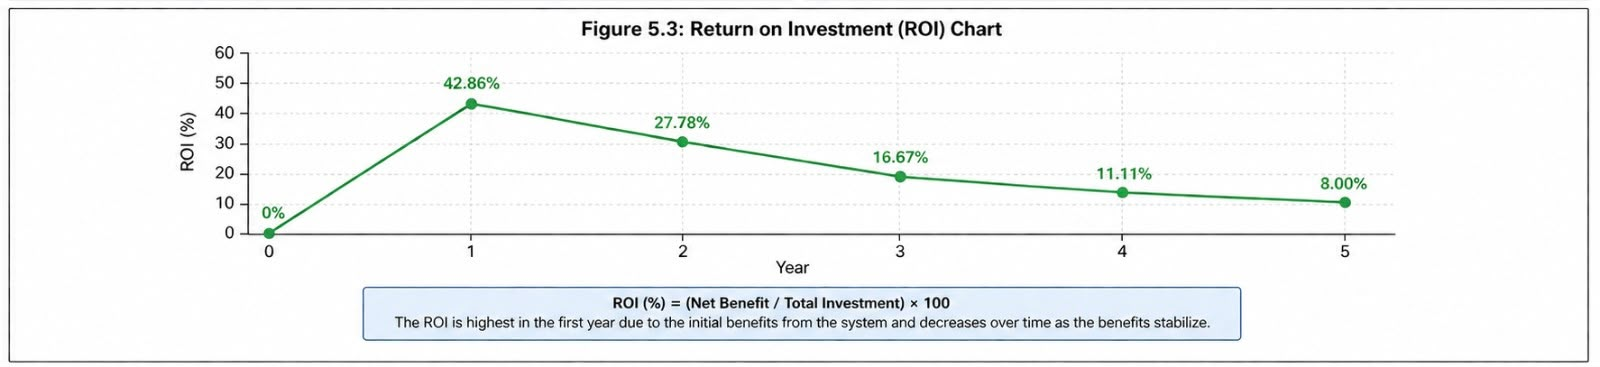
\includegraphics[width=0.75\textwidth]{5.3.jpeg}
    \caption{Return on Investment (ROI) Chart}
\end{figure}
\section{Financial Feasibility Conclusion}

The finance analysis shows that the proposed AI-Integrated Women’s Healthcare Management System looks economically feasible, based on the assumptions used here for this academic project. The estimated development and ongoing costs are balanced, more or less, by expected gains in productivity and administrative savings across the whole project lifecycle. With a positive Net Present Value of USD 5,953.93 and a Return on Investment of 42.86\% , it suggests the system could bring long-term benefit while also improving the way healthcare services are delivered and supporting AI-assisted breast cancer diagnostics.

\end{document}
